% !TeX program = xelatex
% =====================================================================
%  N. Seiberg, E. Witten
%  Electric-Magnetic Duality, Monopole Condensation, And Confinement
%  In N=2 Supersymmetric Yang-Mills Theory
%  arXiv:hep-th/9407087v1 — 中文译注本
%
%  编译：xelatex（两遍；推荐 latexmk -xelatex）
%  依赖：ctex（fontset=fandol）、amsmath、amssymb、amsthm、mathtools、bm、
%        graphicx、xcolor、booktabs、array、enumitem、caption、hyperref
% =====================================================================
\documentclass[11pt,a4paper,UTF8,fontset=fandol]{ctexart}

% ---------- 页面与版式 ----------
\usepackage[a4paper,left=2.6cm,right=2.6cm,top=2.6cm,bottom=2.8cm]{geometry}
\usepackage{fancyhdr}
\pagestyle{fancy}
\fancyhf{}
\fancyhead[L]{\footnotesize\itshape Electric-Magnetic Duality, Monopole Condensation,
  and Confinement}
\fancyhead[R]{\small\thepage}
\renewcommand{\headrulewidth}{0.4pt}
\setlength{\headheight}{14pt}

% ---------- 数学 ----------
\usepackage{amsmath}
\usepackage{amssymb}
\usepackage{amsthm}
\usepackage{mathtools}
\usepackage{bm}

% ---------- 图形、颜色、表格、列表 ----------
\usepackage{graphicx}
\usepackage{xcolor}
\usepackage{booktabs}
\usepackage{array}
\usepackage{enumitem}
\usepackage{caption}
\captionsetup{font=small,labelsep=quad}
\setlength{\emergencystretch}{3em}

% ---------- 超链接 ----------
\usepackage[colorlinks=true,linkcolor=blue!55!black,citecolor=blue!55!black,
            urlcolor=blue!55!black,unicode]{hyperref}

% ---------- 定理类环境 ----------
\theoremstyle{plain}
\newtheorem{theorem}{定理}[section]
\newtheorem{proposition}[theorem]{命题}
\newtheorem{lemma}[theorem]{引理}
\newtheorem{corollary}[theorem]{推论}
\theoremstyle{definition}
\newtheorem{definition}[theorem]{定义}
\newtheorem{remark}[theorem]{注}
\renewcommand{\proofname}{证明}

% ---------- 每节重点（Key Takeaways） ----------
\newenvironment{keypoints}{%
  \par\addvspace{0.9em}%
  \noindent\begin{minipage}{\linewidth}%
  \color{black!80}\rule{\linewidth}{0.6pt}\par\vspace{2pt}%
  \noindent\textbf{【本节重点】}\par\vspace{2pt}%
  \begin{itemize}[leftmargin=1.6em,itemsep=1pt,topsep=2pt,parsep=0pt]%
}{%
  \end{itemize}\vspace{1pt}\noindent\color{black!80}\rule{\linewidth}{0.6pt}%
  \end{minipage}\par\addvspace{0.9em}%
}

% ---------- 常用记号 ----------
\newcommand{\R}{\mathbb{R}}
\newcommand{\C}{\mathbb{C}}
\newcommand{\Z}{\mathbb{Z}}
\newcommand{\dd}{\mathrm{d}}
\newcommand{\ee}{\mathrm{e}}
\newcommand{\ii}{\mathrm{i}}
\newcommand{\Tr}{\operatorname{Tr}}
\newcommand{\tr}{\operatorname{tr}}
\renewcommand{\Re}{\operatorname{Re}}
\renewcommand{\Im}{\operatorname{Im}}
\newcommand{\diag}{\operatorname{diag}}
\newcommand{\id}{\mathrm{id}}
\newcommand{\Nc}{\mathcal{N}}
\newcommand{\Ff}{\mathcal{F}}
\newcommand{\Mm}{\mathcal{M}}
\newcommand{\Hh}{\mathcal{H}}
\newcommand{\Zz}{\mathcal{Z}}
\newcommand{\Ll}{\mathcal{L}}
\newcommand{\Tt}{\mathcal{T}}
\newcommand{\Dd}{\mathcal{D}}
\newcommand{\Ss}{\mathcal{S}}
\newcommand{\Pp}{\mathcal{P}}
\newcommand{\Kk}{\mathcal{K}}
\newcommand{\Uu}{\mathcal{U}}
\newcommand{\Vv}{\mathcal{V}}
\newcommand{\Ww}{\mathcal{W}}
\newcommand{\Aa}{\mathcal{A}}
\newcommand{\Bb}{\mathcal{B}}
\newcommand{\Cc}{\mathcal{C}}
\newcommand{\Ee}{\mathcal{E}}
\newcommand{\Gg}{\mathcal{G}}
\newcommand{\Ii}{\mathcal{I}}
\newcommand{\Jj}{\mathcal{J}}
\newcommand{\Oo}{\mathcal{O}}
\newcommand{\Qq}{\mathcal{Q}}
\newcommand{\Xx}{\mathcal{X}}
\newcommand{\Yy}{\mathcal{Y}}
\newcommand{\fg}{\mathfrak{g}}
\newcommand{\fh}{\mathfrak{h}}
\newcommand{\ft}{\mathfrak{t}}

% PDF 书签中不能出现数学命令，统一降级为纯文本
\pdfstringdefDisableCommands{%
  \def\Nc{N}%
}

% =====================================================================
%  前置部分：标题、摘要、译者说明、目录
%  （由 build.py 以 \input 方式并入主文件；编译请用 xelatex）
% =====================================================================
\begin{document}
\sloppy

\begin{center}
  {\LARGE\bfseries 电磁对偶、磁单极子凝聚与\\[4pt]
   $\mathcal{N}=2$ 超对称杨--米尔斯理论中的禁闭}\\[10pt]
  {\large\itshape Electric-Magnetic Duality, Monopole Condensation,
   and Confinement\\[2pt]
   in $\mathcal{N}=2$ Supersymmetric Yang-Mills Theory}\\[20pt]
  {\large N. Seiberg}\\[4pt]
  {\small Department of Physics and Astronomy, Rutgers University,
   Piscataway, NJ 08855-0849, USA\\
   与 Institute for Advanced Study, Princeton, NJ 08540, USA}\\[10pt]
  {\large E. Witten}\\[4pt]
  {\small Institute for Advanced Study, Princeton, NJ 08540, USA}\\[16pt]
  {\small arXiv:hep-th/9407087v1 [hep-th]，1994 年 7 月 15 日；
   RU-94-52，IAS-94-43\\[2pt]
   中文译注本}
\end{center}
\vspace{6pt}
\hypersetup{pdftitle={电磁对偶、磁单极子凝聚与 N=2 超对称杨-米尔斯理论中的禁闭},
  pdfauthor={N. Seiberg, E. Witten; 中文译注}}

\begin{abstract}
\noindent
我们研究四维 $\mathcal{N}=2$ 超对称规范理论（规范群为 $SU(2)$）的真空结构与双荷子谱。
这一理论具有极其丰富而物理的性质，却仍能被精确描述：例如，电子与双荷子的质量、以及
真空模空间上的度规，都可以得到精确公式。这一描述涉及 Olive--Montonen 电磁对偶的一个
版本。所谓“强耦合”真空，其实是一个磁单极子的弱耦合理论；在适当的微扰下，禁闭由磁单
极子凝聚来描述。
\end{abstract}

\section*{译者说明}
\addcontentsline{toc}{section}{译者说明}

\begin{itemize}[leftmargin=1.6em,itemsep=2pt]
  \item \textbf{底本.} 本译文依据 N. Seiberg 与 E. Witten 的
        \emph{Electric-Magnetic Duality, Monopole Condensation, and Confinement in
        $\mathcal{N}=2$ Supersymmetric Yang-Mills Theory}（arXiv:hep-th/9407087v1，
        1994 年 7 月 15 日，45 页）逐页翻译。原书印刷页与本译本的章节、公式编号一一
        对应；页码映射为\textbf{印刷页 $=$ PDF 页 $-1$}（PDF 第 1 页为标题/摘要页）。
  \item \textbf{公式编号.} 全部沿用原文编号（如式 (2.14)、式 (6.30)），采用
        \verb|\tag| 手工标注；正文按“式 (2.14)”的形式引用，便于与英文本对照。
  \item \textbf{审校批注.} 以 \verb|% [Tutor Note: ...]| 形式的 \LaTeX{} 注释插入源码
        （编译后不显示），内容包括：符号与指标易错处、原文的约定与号差、作者省略
        论证之处、原文印刷笔误。建议对照源码阅读；批注分类索引见随附
        \verb|审校批注汇总.md|。
  \item \textbf{术语与记号.} 译名以国内理论物理界的通行译法为准（规范场、预势、模空间、
        磁单极子、双荷子、单值性等）；人名与模型名保留拉丁字母。冻结术语表与记号表见
        随附 \verb|README.md|。
  \item \textbf{插图.} 原文共两幅插图（原书 p.28 的图 1、p.38 的图 2），已从 PDF 中裁出
        并插入正文对应位置，图注译为中文并标注原书页码。
  \item \textbf{编译.} 请使用 \texttt{XeLaTeX}（或 \verb|latexmk -xelatex|）编译两遍；
        中文排版依赖 \verb|ctex| 宏包，本稿用 \verb|fontset=fandol|，无需额外中文字体。
\end{itemize}

\tableofcontents
\newpage


% ===== 片段：sections/s01.tex =====

\section{引言}
\begin{keypoints}
  \item \textbf{目标：} 用全纯性加电磁对偶，精确求解四维 $\Nc=2$、规范群 $SU(2)$ 的超对称
        杨--米尔斯理论的低能有效理论，包括预势、真空模空间度规与 BPS 谱。
  \item \textbf{工具：} 低能有效超势（预势）对超场与耦合参数的全纯性；超对称代数的中心
        扩张与 BPS 界；$SL(2,\Z)$ 在 $\tau=\theta/2\pi+i4\pi/g^2$ 上的对偶作用。
  \item \textbf{主结论：} 量子模空间的拓扑不变，但几何、奇点结构与物理诠释剧变；“强耦合”
        真空等价于磁单极子的弱耦合理论，磁单极子凝聚给出电荷禁闭。
  \item \textbf{对照 $\Nc=4$：} $\Nc=4$ 有天然的无量纲耦合与 $\theta$ 角，Olive--Montonen
        对偶可能精确成立；$\Nc=2$ 渐近自由、无微观 $\theta$ 角，只有“一个版本”的对偶。
\end{keypoints}

四维 $\Nc=1$ 超对称规范理论的动力学已被广泛研究，部分原因是它可能有现象学上的意义。
近来，人们得到了关于其强耦合行为的一些结果 [1--4]。这些结果在很大程度上是如下事实的
推论：低能有效超势对手征超场以及基础拉格朗日量中的参数都是全纯的 [1]（这种全纯性
的其他方面在 [5,6] 中讨论过）。% [Tutor Note: 全纯性是 Seiberg 在 [1] 中提出的核心工具：\\
% 有效超势作为手征超场与耦合常数的全纯函数，其形式受对称性与奇点行为强烈约束，
% 常常可以被唯一确定。这里“对参数全纯”指把耦合常数（如 $1/g^2$、$\theta$）解析延拓为
% 复参数后，超势仍全纯。]
把超势在其奇点附近的行为与对称性、全纯性结合起来，往往就能精确确定超势。由此得到的
超势有时会展现新的物理现象 [2--4]，这些现象也可能适用于非超对称规范理论。

本文的目标之一，是获得相应的 $\Nc=2$ 理论的类似强耦合信息，至少对最基本的、不含物质
多重态的 $SU(2)$ 规范理论是如此。（这类多重态将在后续论文 [7] 中纳入。）在 $\Nc=2$
理论中，凯勒势与稳定粒子的质量由一个全纯对象——“预势”——控制。因此，可以沿着与
$\Nc=1$ 理论中确定超势大致类似的思路来研究它们，并最终把预势完全确定下来。

尽管我们的结果是在 $\Nc=2$ 超对称这一特殊情形下导出的，它们所展现的物理现象却具有
普遍意义：渐近自由、手征对称性破缺、由强耦合产生质量标度、通过磁单极子凝聚实现电荷
禁闭，以及一个版本的电磁对偶。这些结果也可能有助于理解 $\Nc=4$ 理论中的现象，甚至
弦论中的现象，并有助于理解由 $\Nc=2$ 理论经扭曲而得到的拓扑场论 [8,9]。

由于电磁对偶在求解该模型时将起重要作用，我们在此先回顾一些背景。这类对偶在超对称
杨--米尔斯理论中的存在，最初是从双荷子的性质猜到的——双荷子是同时带电荷与磁荷的
粒子，在 $\Nc=2$ 与 $\Nc=4$ 规范理论的经典层面就已存在。在半经典层面，借由最早源于
Prasad 与 Sommerfield [10] 以及 Bogomol'nyi [11] 的论证，可以求得磁荷与电荷量子数为
$(n_m,n_e)$ 的双荷子满足
\begin{equation}
  M\ge \sqrt{2}\,|Z| \tag{1.1}
\end{equation}
其中
\begin{equation}
  Z=v\left(n_e+i\,\frac{1}{\alpha}\,n_m\right). \tag{1.2}
\end{equation}
这里 $v$ 是希格斯场的期望值，$\alpha=g^2/4\pi$，$g$ 是规范耦合常数。\footnote{我们如此
归一化希格斯场：其动能项乘以 $\dfrac{1}{4\pi\alpha}=\dfrac{1}{g^2}$。}
使 (1.1) 中等号成立的状态称为 BPS 饱和的。要看出量子力学上为何也必定有类似的不等式，
可以把该不等式解释为超对称代数中心扩张的推论 [12]：后面我们会看到，中心扩张中的参数
（从而出现在 $Z$ 定义中的参数）在 $\Nc=2$ 理论中有有趣的重整化，而在 $\Nc=4$ 理论中
没有。% [Tutor Note: (1.1) 中的 $\sqrt2$ 来自手征多重态（chiral multiplet）的归一化约定，
% 与 $\Nc=1$ 超场的动能项归一化有关；换成其他超场归一化时，$\sqrt2$ 会随之改变，
% 但 $M^2=2|Z|^2$ 这一结构不变。式 (1.2) 中 $Z$ 的实部对应电荷 $n_e$、虚部对应磁荷 $n_m$，
% 因此 $|Z|$ 只依赖两者的组合；$Z$ 本身带有 $\alpha=g^2/4\pi$ 归一化，
% 这一点在 §4 讨论 $Z$ 的重整化时很关键。]

质量公式 (1.2) 在 $n_e\leftrightarrow n_m$、$\alpha\leftrightarrow 1/\alpha$、
$v\leftrightarrow v/\alpha$ 之下具有对称性。Olive 与 Montonen [13] 指出了这一对称性，
并猜测它是某个适当量子理论的精确性质。按照这一大胆猜测，理论的强耦合极限等价于把
普通粒子与孤子互换之后的弱耦合极限。$\Nc=2$ 理论看来并不具有 Olive--Montonen 对偶，
因为电子与磁单极子具有不同的洛伦兹量子数（电子处于自旋 $\le 1$ 的超对称多重态中，
而磁单极子的自旋 $\le 1/2$）。另一方面 [14]，对 $\Nc=4$ 理论，电子与磁单极子具有
相同的量子数，这使得 Olive--Montonen 对偶更为可信。事实上，本文将会发现，
Olive--Montonen 对偶的一个版本对 $\Nc=2$ 理论成立。

这一版本必然与 $\Nc=4$ 理论中看似成立的那个版本相当不同。$\Nc=2$ 理论是渐近自由的，
因此耦合常数等价于标度的选择。而且 $U(1)_R$ $R$ 对称性中的反常，阻碍了物理的微观
$\theta$ 角的存在。（低能处仍然有一个有效 $\theta$ 角。）对 $\Nc=4$ 理论，共形不变性与
$U(1)$ 对称性中的反常都相互抵消，因此理论既有天然的无量纲规范耦合 $g$，又有 $\theta$
角；Olive--Montonen 对偶应推广为 $SL(2,\Z)$ 在
$\tau=\dfrac{\theta}{2\pi}+i\,\dfrac{4\pi}{g^2}$ 上的作用——这一点最早是在格点模型
[15,16] 与弦论 [17] 中认识到的。（最近，在多磁单极子束缚态 [18,19] 以及各种流形上的
配分函数 [20,21] 的考虑中，出现了支持这一点的引人注目的新证据。）对 $\Nc=2$ 理论，
这些天然的无量纲参数并不存在；我们所理解的“对偶”，与理论作为希格斯场期望值的函数的
行为有关。
% [Tutor Note: 原书此处只在行文中写出 $\tau=\theta/2\pi+i4\pi/g^2$，没有给它编号，
% 本译本照原文不编号。]
% [Tutor Note: 注意 $\Im\tau=4\pi/g^2>0$，它保证模空间凯勒度规的正定性（见式 (3.10)
% 与 §6 式 (6.4)(6.5)）。$SL(2,\Z)$ 由 $T:\tau\to\tau+1$（即 $\theta\to\theta+2\pi$）
% 与 $S:\tau\to-1/\tau$（电磁对偶）生成；$S$ 在 $\Nc=2$ 理论中不是对称性，而是把一种
% 描述映为同一理论的另一种描述，见 §3.2 式 (3.21)。]

本文的组织如下。第 2 节回顾关于 $\Nc=2$ 超对称规范理论的一些已知事实。经典理论有一族
连续的不等价基态——“经典模空间”。量子修正不会提升真空简并，因此量子理论同样有一族
不等价的基态——“量子模空间”。我们为轻的自由度构造低能有效拉格朗日量。如 [22] 所述，
量子模空间上的度规是凯勒度规，它局部地由一个全纯函数写出。在某些 $\Nc=1$ 模型 [2] 中，
量子修正会改变模空间的拓扑。对 $\Nc=2$ 理论，我们将论证拓扑不变，但几何、奇点结构与
物理诠释会发生显著变化。

在第 3 节，我们更全面地分析低能拉格朗日量的几何。其局部结构只在某一类变换下唯一
（这类变换是某些超引力与弦论中出现的“特殊几何”变换 [23--26] 的平直空间极限）。物理上
它们对应于低能场上的对偶变换。低能拉格朗日量被映射为对偶场的另一个拉格朗日量。

在第 4 节，我们利用轻场与有质量双荷子的耦合，求出双荷子质量的表达式。它包含对经典
结果的量子修正，并且是显式对偶的。我们还（沿着先前的一个二维分析 [27]）描述 BPS 饱和态
（即满足 BPS 质量公式 (1.2) 的态）的谱不发生连续变化的那些条件。这一现象的可能性，最终
成为 $\Nc=2$ 与 $\Nc=4$ 之间的一个本质差别。

在第 5、6 节，我们给出求解模型的方案。第 5 节开头说明：要在量子模空间上得到合理的
凯勒度规，强耦合区至少需要两个奇点。我们提出，这些奇点出现在磁单极子或双荷子质量趋于
零之处。作为检验，我们证明：在进一步的微扰下，磁单极子的凝聚恰好发生在预期电荷禁闭的
地方。这第一次给出了一个真实的相对论场论模型，其中电荷禁闭以这种长期被猜想的机制得到
解释。我们还证明，由无质量磁单极子与双荷子产生的单值性恰好彼此吻合。随后第 6 节证明：
在假定奇点来自无质量磁单极子与双荷子的前提下，可以得到模空间上唯一的度规（以及粒子
质量的唯一公式），且满足全部必要条件。



% ===== 片段：sections/s02.tex =====

\section{$\mathcal N=2$ 超对称的回顾}

\begin{keypoints}
\item $\mathcal N=2$ 理论都带整体 $SU(2)_R$ 对称性；标度不变时还多一个 $U(1)_R$。基本多重态有两类：矢量多重态 $(A_\mu,\lambda,\psi,\phi)$ 与超多重态 $(q,\tilde q^\dagger,\psi_q,\psi^\dagger_{\tilde q})$，在 $\mathcal N=1$ 语言中分别拆成“矢量加手征”与“两个手征”。
\item 纯 $\mathcal N=2$ 理论的经典势为 $V=\frac{1}{g^2}\operatorname{Tr}[\phi,\phi^\dagger]^2$，只要 $\phi$ 与 $\phi^\dagger$ 对易，势就为零，故经典真空构成一族模空间；$SU(2)$ 情形由 $u=\frac12 a^2=\operatorname{Tr}\phi^2$ 标记。
\item 低能有效拉格朗日量只由一个全纯预势 $\mathcal F(\mathcal A)$ 决定：有效耦合为 $\tau=\partial^2\mathcal F/\partial a^2$，凯勒势与度规也由 $\mathcal F$ 给出，见式 (2.8)–(2.10)。
\item 量子修正不解除真空简并，量子模空间仍是凯勒流形；经典公式 $\mathcal F_0=\frac12\tau_{\rm cl}\mathcal A^2$ 只在 $a$ 很大时成立，$a\to 0$ 附近的行为完全不同。
\end{keypoints}

\subsection{表示}

所有 $\mathcal N=2$ 理论都有一个整体 $SU(2)_R$ 对称性，它作用在给定手征性的两个超荷上。标度不变的 $\mathcal N=2$ 理论还有 $U(1)_R$ 对称性，在其中正手征性的超荷带荷 $-1$。

我们将研究两类 $\mathcal N=2$ 多重态。

\begin{enumerate}
\item 第一类是 $\mathcal N=2$ 手征多重态（有时称为矢量多重态），包含规范场 $A_\mu$、两个 Weyl 费米子（外尔费米子）$\lambda$ 与 $\psi$，以及一个标量 $\phi$，它们全都处在伴随表示中。我们把场排成

\begin{equation}
\begin{gathered}
A_\mu\\[2pt]
\lambda\qquad\psi\\[2pt]
\phi
\end{gathered}\tag{2.1}
\end{equation}

以体现 $SU(2)_R$ 对称性：它作用在行上，$A_\mu$ 与 $\phi$ 是单态，$\lambda,\psi$ 构成双重态。用 $\mathcal N=1$ 超对称的语言，这些场可以组织成一个矢量多重态 $W_\alpha$（含 $(A_\mu,\lambda)$）与一个手征多重态 $\Phi$（含 $(\phi,\psi)$）。在这个表述里，$SU(2)_R$ 的生成元中只有一个是显现出来的，我们称它为 $U(1)_J$。$U(1)_J$ 与 $U(1)_R$ 都是 $\mathcal N=1$ 的 $R$ 对称性，作用方式为

\begin{equation}
\begin{aligned}
U(1)_J:\quad \Phi &\to \Phi(e^{-i\alpha}\theta)\\[2pt]
U(1)_R:\quad \Phi &\to e^{2i\alpha}\Phi(e^{-i\alpha}\theta)\,.
\end{aligned}\tag{2.2}
\end{equation}

% [Tutor Note: 易错预警｜式 (2.2)（印刷 p.4）：括号里的 $\theta$ 是超空间坐标，$e^{-i\alpha}\theta$ 表示对超场作坐标重标度，并非把 $\Phi$ 乘以一个数。若误当乘法，$U(1)_J$ 与 $U(1)_R$ 的荷分配会全部错位。$U(1)_J$ 是 $SU(2)_R$ 的 Cartan 生成元；$U(1)_R$ 才是独立的那一个。]

\item 第二类多重态是超多重态（hypermultiplet，有时称为标量多重态），它由两个 Weyl 费米子 $\psi_q$ 与 $\psi^\dagger_{\tilde q}$，以及复玻色子 $q$ 与 $\tilde q^\dagger$ 组成；$SU(2)_R$ 同样作用在菱形的行上：

\begin{equation}
\begin{gathered}
\psi_q\\[2pt]
q\qquad\tilde q^\dagger\,.\\[2pt]
\psi^\dagger_{\tilde q}
\end{gathered}\tag{2.3}
\end{equation}

用 $\mathcal N=1$ 超对称的语言，这些场组成两个手征多重态 $Q$ 与 $\tilde Q$。(2.2) 中的对称性对它们的作用为

\begin{equation}
\begin{aligned}
U(1)_J:\quad Q &\to e^{i\alpha}Q(e^{-i\alpha}\theta)\\
\tilde Q &\to e^{i\alpha}\tilde Q(e^{-i\alpha}\theta)\\[2pt]
U(1)_R:\quad Q &\to Q(e^{-i\alpha}\theta)\\
\tilde Q &\to \tilde Q(e^{-i\alpha}\theta)
\end{aligned}\tag{2.4}
\end{equation}

$\tilde Q$ 的规范量子数与 $Q$ 的规范量子数互为对偶。

% [Tutor Note: 易错预警｜式 (2.3)（印刷 p.5）：菱形中间一行是 $q$ 与 $\tilde q^\dagger$，不是 $q$ 与 $\tilde q$；底部是 $\psi^\dagger_{\tilde q}$，波浪号在下标 $q$ 上而不在 $\psi$ 上。这正对应 $\mathcal N=1$ 分解 $Q=(q,\psi_q)$、$\tilde Q=(\tilde q,\psi_{\tilde q})$：中间一行放的是 $Q$ 的标量分量与 $\tilde Q$ 标量分量的复共轭，两个手征多重态是交错排列的。]
\end{enumerate}

\subsection{可重整拉格朗日量与经典平坦方向}

我们考虑一个 $\mathcal N=2$ 规范理论，它由规范群 $G$ 的伴随表示中的手征超场描述，可能还耦合额外的物质超多重态。$\mathcal N=2$ 超对称把规范耦合与某些相互作用联系起来，而在 $\mathcal N=1$ 的语言中这些相互作用由超势描述。事实上，超势里必需的项是（采用 [28] 的记号）

\begin{equation}
W=\sqrt2\,\tilde Q\Phi Q\,.\tag{2.5}
\end{equation}

这是合理的：$\tilde Q$ 与 $Q$ 变换在对偶表示中，而 $\Phi$ 处在伴随表示。

经典上，拉格朗日量在 $SU(2)_R\times U(1)_R$ 对称性 (2.2)、(2.4) 下不变；此外视超多重态所处的规范表示，还可能在若干味对称性下不变。在量子理论中，$U(1)_R$ 对称性一般被反常破坏。对于带有 $N_f$ 个基础表示无质量超多重态（“夸克”）的 $SU(N_c)$ 规范理论，$U(1)_R$ 破缺为 $\mathbf Z_{4N_c-2N_f}$。

本文主要考虑不带夸克的 $SU(2)$ 规范理论。此时整体对称性是 $(SU(2)_R\times\mathbf Z_8)/\mathbf Z_2$，因为 $4N_c-2N_f=8$（除以 $\mathbf Z_2$ 是因为 $SU(2)_R$ 的中心包含在 $\mathbf Z_8$ 里）。

纯 $\mathcal N=2$ 理论（不含超多重态）的经典势为

\begin{equation}
V(\phi)=\frac{1}{g^2}\operatorname{Tr}[\phi,\phi^\dagger]^2\,.\tag{2.6}
\end{equation}

要使这个势为零，不必让 $\phi$ 本身为零；只要 $\phi$ 与 $\phi^\dagger$ 对易就够了。因此经典理论有一族真空态。例如规范群为 $SU(2)$ 时，相差一个规范变换可以取 $\phi=\frac12a\sigma^3$，其中 $\sigma^3=\operatorname{diag}(1,-1)$，$a$ 是标记真空的复参数。$SU(2)$ 的 Weyl 群作用为 $a\leftrightarrow -a$，因此参数化真空空间的规范不变量是 $u=\frac12a^2=\operatorname{Tr}\phi^2$。当 $a\neq 0$ 时，规范对称性破缺为 $U(1)$，整体 $\mathbf Z_8$ 对称性破缺为 $\mathbf Z_4$。由于 $u$ 的 $U(1)_R$ 荷为 4，残余的 $\mathbf Z_4$ 在 $u$ 平面上平凡地作用。整体对称群在 $u$ 平面上表现为一个自发破缺的 $\mathbf Z_2$，其作用是 $u\leftrightarrow -u$。

经典上，$u=0$ 处有一个奇点：那里完整的 $SU(2)$ 规范对称性恢复，更多场变成无质量。

% [Tutor Note: 背景直觉｜式 (2.6)（印刷 p.6）：这是 $\mathcal N=2$ 矢量多重态的 D 项势 $\propto\operatorname{Tr}D^2$ 消去辅助场后的形式，量纲为四。它只在 $\phi$ 与 $\phi^\dagger$ 的对易子为零时为零，这就是“经典平坦方向”的来源；复维数为 1 的平坦方向随后被 $u$ 参数化。

% [Tutor Note: 易错预警｜$u=\frac12a^2=\operatorname{Tr}\phi^2$（印刷 p.6）：由 $\phi=\frac12a\sigma^3$、$\operatorname{Tr}(\sigma^3)^2=2$ 得 $\operatorname{Tr}\phi^2=\frac{a^2}{4}\cdot2=\frac12a^2$。若把 $\operatorname{Tr}$ 的归一化或 $\sigma^3$ 的归一化换掉，系数会差 2；本节全部 $u$ 依赖都建立在这个 $\frac12$ 上。]

% [Tutor Note: 含糊点拨｜$u\leftrightarrow -u$ 段（印刷 p.6）：作者只说整体对称群“表现为自发破缺的 $\mathbf Z_2$”，没有点明它的来源。它来自被 $a$ 破缺的 $\mathbf Z_8/\mathbf Z_4$ 陪集：$u$ 带 $U(1)_R$ 荷 4，而 $\mathbf Z_8$ 的生成元对 $a$ 的作用是 $a\to ia$，于是 $a^2\to -a^2$，即 $u\to-u$。另外注意规范 Weyl 群给出的 $a\leftrightarrow-a$ 不改变 $u$，不要和这个整体 $\mathbf Z_2$ 混淆。]

\subsection{低能有效作用量}

现在研究模空间上轻场的低能有效作用量。对于一般的 $\langle\phi\rangle$，低能有效拉格朗日量只包含一个 $\mathcal N=2$ 矢量多重态 $\mathcal A$。至多含两个导数、不超过四个费米子的那些项受 $\mathcal N=2$ 超对称限制，可以用单个全纯函数 $\mathcal F(\mathcal A)$ 表示，见 [22]。在 $\mathcal N=1$ 超空间中，拉格朗日量为

\begin{equation}
\frac{1}{4\pi}\operatorname{Im}\left[\int \mathrm{d}^4\theta\,\frac{\partial\mathcal F(A)}{\partial A}\bar A+\int \mathrm{d}^2\theta\,\frac12\frac{\partial^2\mathcal F(A)}{\partial A^2}W_\alpha W^\alpha\right]\tag{2.7}
\end{equation}

其中 $A$ 是 $\mathcal N=2$ 矢量多重态 $\mathcal A$ 里的 $\mathcal N=1$ 手征多重态，其标量分量为 $a$。

我们作几点评论。

\begin{enumerate}
\item 当 $a$ 很大时，渐近自由起作用，理论是弱耦合的。此外，由于不可能给 (2.7) 加上 $\mathcal N=2$ 不变的超势，真空简并在量子层面无法被消除。因此量子理论有一个非平凡的模空间，它实际上是一个复一维的凯勒流形。凯勒势可以用低能有效的 $\mathcal F$ 函数写成

\begin{equation}
K=\operatorname{Im}\left(\frac{\partial\mathcal F(A)}{\partial A}\bar A\right).\tag{2.8}
\end{equation}

于是度规具体为

\begin{equation}
(\mathrm{d}s)^2=\operatorname{Im}\frac{\partial^2\mathcal F(a)}{\partial a^2}\,\mathrm{d}a\,\mathrm{d}\bar a\,.\tag{2.9}
\end{equation}

经典理论中，$\mathcal F$ 可以从 $SU(2)$ 规范理论的树图级拉格朗日量读出，即 $\mathcal F(\mathcal A)=\frac12\tau_{\rm cl}A^2$，其中 $\tau_{\rm cl}=\frac{\theta}{2\pi}+i\frac{4\pi}{g^2}$。渐近自由意味着，只要把 $g^2$ 换成合适的有效耦合，这个公式在 $a$ 很大时就成立。但 $a$ 很小时的行为将完全不同。经典上，$\theta$ 参数没有任何可观测后果。量子层面物理依赖于 $\theta$，不过由于存在一个反常对称性，$\theta$ 可以吸收进场的重新定义里。因此我们取 $\theta=0$。

\item 凯勒势的这个公式看起来并不协变——只有在一类特殊的坐标系中，凯勒势才能写成这种形式，而这些坐标系我们稍后会分析。事实上，$A$ 通过 $\mathcal N=2$ 超对称与“光子” $A_\mu$ 相联系，后者具有自然的线性结构；这就为 $A$ 提供了一个自然坐标系（或者说，之后会证明是一类自然的坐标系）。

\item 规范耦合常数与 $\theta$ 参数的低能取值可以从拉格朗日量读出。若把它们组合成 $\tau=\frac{\theta}{2\pi}+i\frac{4\pi}{g^2}$，并把由 $a$ 参数化的真空中的有效耦合记为 $\tau(a)$，则

\begin{equation}
\tau(a)=\frac{\partial^2\mathcal F}{\partial a^2}\,.\tag{2.10}
\end{equation}

\item 推广到任意秩为 $r$ 的紧致规范群 $G$ 如下。势总是由 (2.6) 给出，因此经典真空由满足 $[\phi,\phi^\dagger]=0$ 的伴随值复矩阵 $\phi$ 标记。模空间一般点处未破缺的规范对称性是 Cartan 子代数，因此模空间的复维数为 $r$。低能理论用 $r$ 个阿贝尔手征多重态 $\mathcal A^i$ 描述，(2.7) 的推广是 [22]

\begin{equation}
\frac{1}{4\pi}\operatorname{Im}\left[\int \mathrm{d}^4\theta\,\frac{\partial\mathcal F(A)}{\partial A^i}\bar A^i+\int \mathrm{d}^2\theta\,\frac12\frac{\partial^2\mathcal F(A)}{\partial A^i\partial A^j}W^i_\alpha W^{\alpha j}\right].\tag{2.11}
\end{equation}

这里 $i$ 标记 Cartan 子代数中的生成元，而局部地 $\mathcal F$ 是 $r$ 个复变量的任意全纯函数。

\item $SU(2)$ 理论在 $u\neq 0$ 的平坦方向上研究时，除了无质量的手征/矢量多重态 $\mathcal A$，还有额外的带电有质量矢量多重态。对三重手征多重态 $\mathcal A^a$（$a=1\ldots 3$）很容易写出一个规范不变的有效作用量，它在低能下对无质量场约化为 (2.7)，同时把有质量场也包含进来。

沿用上面的同一个函数 $\mathcal F$，令 $\mathcal F(\sqrt{\mathcal A\cdot\mathcal A})=\mathcal H(\mathcal A\cdot\mathcal A)$，并写下

\begin{equation}
\frac{1}{2\pi}\operatorname{Im}\left[\int \mathrm{d}^4\theta\,\mathcal H' A^a (e^V)_{ab}\bar A^b+\int \mathrm{d}^2\theta\,\frac12\left(\mathcal H'\delta^{ab}+2\mathcal H'' A^a A^b\right)W^a_\alpha W^b_\alpha\right]\tag{2.12}
\end{equation}

这里我们用 $SU(2)$ 不变的度规 $\delta^{ab}$ 升降指标。(2.12) 具有 $\mathcal N=2$ 超对称性与显式的规范不变性，并在低能下约化为 (2.7)。

\item 若给 $\mathcal F$ 加上关于 $A$ 线性的项，拉格朗日量 (2.7) 不变。其效果是把 $\partial\mathcal F/\partial A$ 平移一个常数。稍后我们会赋予 $h(A)=\partial\mathcal F/\partial A$ 物理意义：

\begin{equation}
h(A)=\frac{\partial\mathcal F}{\partial A}\,.\tag{2.13}
\end{equation}

这个可加常数总是通过和高能理论比较来确定，如 (2.12) 所示。

正如我们已经提到的，经典上 $\mathcal F$ 函数是

\begin{equation}
\mathcal F_0=\frac12\tau_{\rm cl}\mathcal A^2\,.\tag{2.14}
\end{equation}
\end{enumerate}

% [Tutor Note: 含糊点拨｜式 (2.7)–(2.8)（印刷 p.6–7）：原文在“$\mathcal N=2$ 矢量多重态”用花体 $\mathcal A$、在“$\mathcal N=1$ 手征超场”用斜体 $A$，但两个字号接近，很容易看混。全节的约定是：$\mathcal A$ 指 $\mathcal N=2$ 多重态，$A$ 指它里面的 $\mathcal N=1$ 手征超场，$a$ 是 $A$ 的标量分量；$\mathcal F$ 的导数一律对 $A$ 取。读者若把 (2.7) 的 $A$ 当成 $\mathcal A$，会误以为预势是 $\mathcal N=2$ 超场的函数。]

% [Tutor Note: 易错预警｜式 (2.9)（印刷 p.7）：$\operatorname{Im}$ 作用在二阶导数 $\partial^2\mathcal F/\partial a^2$ 上，$\mathrm{d}a\,\mathrm{d}\bar a$ 是普通乘积而非楔积，因此没有额外的 $1/2$ 或 $i$。此外，凯勒度规的正定性要求 $\operatorname{Im}\tau(a)>0$，这一点在下文用单值性论证 $\operatorname{Im}\tau$ 不可能处处为正时会成为关键。]

% [Tutor Note: 易错预警｜式 (2.11)（印刷 p.8）：与 (2.7) 相比，这里 $\alpha$ 自旋指标收缩在同一对 $W$ 上（$W^i_\alpha W^{\alpha j}$），而 $i,j$ 是 Cartan 子代数的指标，$\mathcal F$ 对 $A^i$ 的二阶偏导给出 $\tau_{ij}$。不要漏掉 $W$ 的 $\alpha$ 上标，否则指标不闭合。]

% [Tutor Note: 含糊点拨｜式 (2.12) 与 (2.7) 的系数（印刷 p.8）：为什么 (2.12) 前面是 $1/2\pi$，而 (2.7) 是 $1/4\pi$？由 $\mathcal F(\sqrt{\mathcal A\cdot\mathcal A})=\mathcal H(\mathcal A\cdot\mathcal A)$ 可得 $\partial\mathcal F/\partial A^a=2\mathcal H'A^a$、$\partial^2\mathcal F/\partial A^a\partial A^b=2\mathcal H'\delta^{ab}+4\mathcal H''A^aA^b$；求导带出的因子 2 恰好与 (2.12) 的 $\frac12$ 及 $1/2\pi$ 相抵，低能下便回到 (2.7)。作者跳过了这一步验证。]

% [Tutor Note: 易错预警｜式 (2.12)（印刷 p.8）：原文末项印作 $W^a_\alpha W^b_\alpha$，两个 $\alpha$ 都在下标，按指标规则应为 $W^a_\alpha W^{b\alpha}$（对照 (2.7)、(2.11) 的写法）。此处照原文排印，属可疑笔误，已记入回报；另外 $\mathcal H'$、$\mathcal H''$ 分别是对自变量 $\mathcal A\cdot\mathcal A$ 的一阶、二阶导数，原文未明言，容易漏读。]

% [Tutor Note: 含糊点拨｜经典预势的两处写法（印刷 p.7–8）：正文写作 $\mathcal F(\mathcal A)=\frac12\tau_{\rm cl}A^2$，括号内是花体 $\mathcal A$、平方项却是斜体 $A$；而编号式 (2.14) 印作 $\mathcal F_0=\frac12\tau_{\rm cl}\mathcal A^2$。判断前者为排印笔误，此处照原样保留，读者应以 (2.14) 为准。]


% ===== 片段：sections/s02b.tex =====

% （承 §2.3：PDF p10 / 印刷 p9 顶部；§2.3 在此结束，其后即 §3 标题）
量子修正已由 [22] 分析过。树图级与单圈贡献相加得到
\begin{equation}
  \Ff_{\text{one loop}}=i\,\frac{1}{2\pi}\,A^2\ln\frac{A^2}{\Lambda^2} \tag{2.15}
\end{equation}
其中 $\Lambda$ 是动力学产生的标度。这个对数与单圈 $\beta$ 函数有关，也保证了在
$U(1)_R$ 下的反常变换律。更高阶的微扰修正不再出现。瞬子会带来新的项；反常与瞬子
作用量提示
\begin{equation}
  \Ff=i\,\frac{1}{2\pi}\,A^2\ln\frac{A^2}{\Lambda^2}
  +\sum_{k=1}^{\infty}\Ff_k\left(\frac{\Lambda}{A}\right)^{4k}A^2 \tag{2.16}
\end{equation}
其中第 $k$ 项来自 $k$ 个瞬子的贡献。对 $k=1$ 项的详细计算 [22] 表明
$\Ff_1\neq 0$。我们很快就会看到，无穷多个 $\Ff_k$ 都非零。
% [Tutor Note: 易错预警｜式 (2.15)(2.16)（印刷 p.9）：$\Ff$ 是预势（作为 $\mathcal N=2$
% 矢量多重态标量分量的全纯函数），不是超势；$A$ 在这里指 $\mathcal N=2$ 手征超场
% （原文在 §2.3 中沿用了 §1 的 $A$ 记号）。单圈系数 $i/2\pi$ 由单圈 $\beta$ 函数定出，
% 它与 $\tau=\partial^2\Ff/\partial A^2$ 的虚部（即 $4\pi/g^2$）一致。
% 展开参数是 $(\Lambda/A)^{4k}$ 而非 $(\Lambda/A)^{k}$：这是 $U(1)_R$ 荷守恒（$A$ 的荷为 2、
% $\Lambda$ 的荷为 $2/3$、瞬子荷为 8）所要求的。]
% [Tutor Note: 含糊点拨｜“反常与瞬子作用量提示”(2.16)（印刷 p.9）：作者未展开的论证是
% 非微扰项必须按 $e^{-8\pi^2/g^2}\sim(\Lambda/A)^4$ 的幂次出现，而 $U(1)_R$ 与量纲分析
% 把每一项唯一地固定成 $\Ff_k(\Lambda/A)^{4k}A^2$；$k$ 即瞬子数。$\Ff_1\neq0$ 的结论
% 来自 [22]（Seiberg 1988）的单瞬子计算。]

对经典公式 (2.14) 的修正与 $\beta$ 函数有关；特别地，对 $\beta$ 函数为零的
$\mathcal N=4$ 超对称杨--米尔斯理论，公式 (2.14) 是精确的。



% ===== 片段：sections/s03.tex =====

\section{对偶}
\begin{keypoints}
  \item \textbf{局部而非整体：} $\Nc=2$ 超对称把真空模空间上的度规写成
        $(\dd s)^2=\Im\tau\,\dd a\,\dd\bar a$，其中 $\tau=\partial^2\Ff/\partial a^2$；
        但 $\Im\tau$ 是调和函数、不可能取到极小值，所以这种描述只能是局部的。
  \item \textbf{对称结构：} 以 $(a_D,a)$ 为辛空间坐标时，保持度规结构的变换构成
        $SL(2,\R)$（还要加上常数平移 $c$），最终约化为 $SL(2,\Z)$；多规范群情形推广为
        $Sp(2r,\R)\to Sp(2r,\Z)$。
  \item \textbf{两个生成元：} $T_b$ 把 $\theta$ 角平移 $2\pi b$，故 $b$ 必须是整数；
        $S$ 就是电磁对偶，它把 $\tau$ 反演成 $-1/\tau$。对偶不是理论的对称性，
        而是同一理论的两种描述之间的转换。
  \item \textbf{对偶化技术：} 用拉格朗日乘子把 $\dd F=0$ 变成约束、再对 $F$ 作高斯积分；
        玻色情形与 $\Nc=1$ 超空间情形分别给出式 (3.12)--(3.14) 与 (3.15)--(3.16)。
  \item \textbf{与引力比较：} 超引力“特殊几何”的凯勒势 (3.26) 在
        $M_{\mathrm{Pl}}\to\infty$ 时约化为整体超对称的 (3.27)，允许的单值性群也一致。
\end{keypoints}

上文中我们已经指出：局部地，由 $\Nc=2$ 超对称，模空间上的度规具有如下形式
\begin{equation}
  (\dd s)^2=\Im\tau(a)\,\dd a\,\dd\bar a, \tag{3.1}
\end{equation}
其中 $\tau(a)$ 是全纯函数 $\tau=\partial^2\Ff/\partial a^2$。单圈公式 (2.15) 表明，当 $|a|$
很大时，$\tau(a)\approx\ii\left(\ln(a^2/\Lambda^2)+3\right)/\pi$ 是一个多值函数，其虚部
单值且为正。然而，若 $\Im\tau(a)$ 能整体地定义，它就不可能正定，因为调和函数 $\Im\tau$
不可能取到极小值。这说明上述度规描述只能在局部成立。
% [Tutor Note: 印刷 p.9，式 (3.1) 前后。这里的论证是复分析里的常识：非常数的调和函数在
% 定义域内部取不到极小值，所以不可能存在处处为正的整体 $\Im\tau$；这正是全节反复
% 出现的“只能局部”的根源。后面 §5、§6 通过引入多个奇点、让 $\Im\tau$ 沿闭合回路单值化，
% 才把模空间整体拼起来。\\]

把变量从 $a$ 换到某个别的局部参数、同时让度规保持 (3.1) 的形式，这件事能做到什么程度？
这个问题的答案正是物理的核心所在。我们定义 $a_D=\partial\Ff/\partial a$，于是度规可以写成
\begin{equation}
  (\dd s)^2=\Im \dd a_D\,\dd\bar a
  =-\frac{\ii}{2}\left(\dd a_D\dd\bar a-\dd a\dd\bar a_D\right). \tag{3.2}
\end{equation}
这个公式对 $a$ 与 $a_D$ 完全对称；因此若改用 $a_D$ 作局部参数，度规就会具有与 (3.1) 相同
的一般形式，只是 $\Im\tau$ 换成了另一个调和函数。我们马上会看到，这个变换对应于电磁对偶。
在进入这一点之前，先让我们弄清：能把度规写成 (3.2) 的局部参数，其全体是什么。
% [Tutor Note: 印刷 p.9--10，式 (3.2)。由 $\dd a_D=\tau\,\dd a$ 可知 (3.1) 与 (3.2) 是同一个
% 度规；改用 $a_D$ 当坐标后，新的复耦合 $\tau_D$ 与 $\tau$ 的关系正是 §3.2 式 (3.21) 的
% $\tau_D=-1/\tau$。所以“换局部参数”与“电磁对偶”在数学上是同一件事：
% 前者只讲度规的凯勒结构，后者才把它提升为对规范场的操作。]

\subsection{数学描述}

为了以对 $a$ 与 $a_D$ 完全对称的方式来处理这套形式，我们引入一个任意的局部全纯坐标 $u$，
把 $a$ 与 $a_D$ 都看作 $u$ 的函数。$u$ 是复流形 $\Mm$ 上的局部坐标，而 $\Mm$ 是该理论的
真空模空间。最终我们会取 $u$ 为 $\Tr\phi^2$ 的期望值——那是一个合适的物理参数——但现在
$u$ 仍是任意的。

引入一个坐标为 $(a_D,a)$ 的二维复空间 $X\cong\C^2$，并赋予 $X$ 辛形式
$\omega=\Im \dd a_D\wedge\dd\bar a$。函数对 $(a_D(u),a(u))$ 给出从 $\Mm$ 到 $X$ 的映射 $f$。
$\Mm$ 上的度规是
\begin{equation}
  (\dd s)^2=\Im\frac{\dd a_D}{\dd u}\frac{\dd\bar a}{\dd\bar u}\dd u\,\dd\bar u
  =-\frac{\ii}{2}\left(\frac{\dd a_D}{\dd u}\frac{\dd\bar a}{\dd\bar u}
  -\frac{\dd a}{\dd u}\frac{\dd\bar a_D}{\dd\bar u}\right)\dd u\,\dd\bar u. \tag{3.3}
\end{equation}
这个公式对 $\Mm$ 上任意局部参数 $u$ 都成立。若取 $u=a$，就回到度规原来的公式 (2.9)。
（上面这个公式可以用坐标无关的说法表述为：$\Mm$ 上诱导度规的凯勒形式是 $f^{\ast}(\omega)$。）
注意 $\omega$ 并不具有任何正性；因此，如果 $a(u)$ 与 $a_D(u)$ 是完全任意的局部全纯函数，
度规 (3.3) 并不正。后面我们会以特定的方式构造 $a(u)$ 与 $a_D(u)$，以保证正性。
% [Tutor Note: 印刷 p.10，式 (3.3)。括号里的两项不要记混：第一项是
% $\frac{\dd a_D}{\dd u}\frac{\dd\bar a}{\dd\bar u}$，第二项是
% $\frac{\dd a}{\dd u}\frac{\dd\bar a_D}{\dd\bar u}$，最后一个 $\dd u\,\dd\bar u$ 在括号外。
% 另外注意 $\omega=\Im \dd a_D\wedge\dd\bar a$ 只是一个辛形式（凯勒形式），它本身没有正性，
% 所以原文紧接着强调 (3.3) 未必正；正性要靠后面具体构造的 $a(u),a_D(u)$ 才能保证。\\]

容易看出，什么样的变换能保持度规的一般结构。令 $a^\alpha=(a_D,a)$，$\alpha=1,2$，再令
$\varepsilon_{\alpha\beta}$ 为满足 $\varepsilon_{12}=1$ 的反对称张量，则
\begin{equation}
  (\dd s)^2=-\frac{\ii}{2}\varepsilon_{\alpha\beta}
  \frac{\dd a^\alpha}{\dd u}\frac{\dd\bar a^\beta}{\dd\bar u}\dd u\,\dd\bar u. \tag{3.4}
\end{equation}
在保持 $\varepsilon$、且与复共轭对易的线性变换下，这个式子明显不变（后一个条件保证
$a^\alpha$ 与 $\bar a^\alpha$ 以相同的方式变换）。这些变换构成群 $SL(2,\R)$（等价地，
也就是 $Sp(2,\R)$）。此外，(3.4) 显然在给 $a_D$ 或 $a$ 加上常数时不变。于是，若把
$(a_D,a)$ 排成列向量 $v$，保持一般结构的对称变换就是
\begin{equation}
  v\to Mv+c, \tag{3.5}
\end{equation}
其中 $M$ 是 $SL(2,\R)$ 中的 $2\times2$ 矩阵，$c$ 是常向量。后面我们会发现（依据涉及
规范场以及电荷与磁荷的考虑），$M$ 必须属于 $SL(2,\Z)$；而且在纯 $\Nc=2$ 规范理论中，
$c$ 必须为零。（在与物质耦合时，$c$ 会起重要作用 [7]。）一般地，变换 (3.5) 构成的群
可以看成由形如
\begin{equation}
  \begin{pmatrix} 1 & 0 \\ c & M \end{pmatrix}, \tag{3.6}
\end{equation}
的 $3\times3$ 矩阵组成的群，它作用在三个对象 $(1,a_D,a)$ 上。
% [Tutor Note: 印刷 p.10--11，式 (3.4)--(3.6)。式 (3.4) 里 $a^1=a_D$、$a^2=a$，
% $\varepsilon_{\alpha\beta}$ 只需由 $\varepsilon_{12}=1$ 定出分量（$\varepsilon_{21}=-1$）。
% 式 (3.6) 是分块写法：顶行 $(1\ \ 0)$ 中的 $0$ 是 $1\times2$ 的零行，底行 $(c\ \ M)$ 中
% $c$ 是 $2\times1$ 列、$M$ 是 $2\times2$ 矩阵；它作用在 $(1,a_D,a)$ 上时，常数项 $c$
% 恰好实现 (3.5) 的平移。纯 $\Nc=2$ 理论为什么 $c=0$、耦合物质时 $c$ 又起什么作用，
% 本文正文不展开，见文献 [7]。\\]

\noindent\textbf{推广到维数大于一}

虽然本文不会用到它、读者也可以略过，我们还是简述一下对其他规范群的推广。若规范群 $G$
的秩为 $r$，则 $\Mm$ 的复维数为 $r$。局部地，由 (2.11)，度规为
\begin{equation}
  (\dd s)^2=\Im\frac{\partial^2\Ff}{\partial a^i\partial a^j}\dd a^i\dd\bar a^j, \tag{3.7}
\end{equation}
其中 $a^i$ 是特殊的局部坐标，$\Ff$ 是全纯函数。我们照旧改写它：引入
\begin{equation}
  a_{D,j}=\frac{\partial\Ff}{\partial a^j}. \tag{3.8}
\end{equation}
于是可以写成
\begin{equation}
  (\dd s)^2=\Im\sum_i \dd a_{D,i}\dd\bar a^i. \tag{3.9}
\end{equation}
为了不变地表述这一套，我们引入坐标为 $a^i,a_{D,j}$ 的复空间 $X\cong\C^{2r}$，并赋予 $X$
一个 $(1,1)$ 型的辛形式
$\omega=\frac{\ii}{2}\sum_i\left(\dd a^i\wedge\dd\bar a_{D,i}
-\dd a_{D,i}\wedge\dd\bar a^i\right)$，以及全纯二形式
$\omega_h=\sum_i \dd a^i\wedge\dd a_{D,i}$。接着在模空间 $\Mm$ 上引入任意局部坐标 $u^s$
（$s=1,\dots,r$），并用函数 $a^i(u),a_{D,j}(u)$ 描述映射 $f:\Mm\to X$。我们要求 $f$
满足 $f^{\ast}(\omega_h)=0$；这恰好保证：局部地，若取 $u^i=a^i$，则 $a_{D,j}$ 必取
(3.8) 的形式，其中 $\Ff$ 是某个全纯函数。然后我们取 $\Mm$ 上的度规为凯勒形式等于
$f^{\ast}(\omega)$ 的那个度规；写成公式就是
\begin{equation}
  (\dd s)^2=\Im\sum_{s,t,i}
  \frac{\partial a_{D,i}}{\partial u^s}\frac{\partial\bar a^i}{\partial\bar u^t}
  \dd u^s\dd\bar u^t. \tag{3.10}
\end{equation}
若再把 $a,a_D$ 排成 $2r$ 分量的列向量 $v$，则这套形式在变换 $v\to Mv+c$ 下不变，其中
$M$ 是 $Sp(2r,\R)$ 中的矩阵，$c$ 是常向量。同样，涉及电荷的考虑最终会要求 $M$ 属于
$Sp(2r,\Z)$，并对 $c$ 施加限制。
% [Tutor Note: 印刷 p.11--12，式 (3.7)--(3.10)。式 (3.7) 原文没有写求和号，按 Einstein
% 约定对 $i,j$ 求和；$a_{D,i}$ 的下标与 $a^i$ 的上标配对，是本文全篇的指标约定。
% 式 (3.10) 里 $s,t,i$ 三重求和，$u^s$ 是模空间 $\Mm$ 上的坐标而非特殊坐标。条件
% $f^{\ast}(\omega_h)=0$ 是“可积性”条件：它保证 $\tau_{ij}$ 真能写成某个预势的二阶导数
% $\partial_i\partial_j\Ff$，从而 (3.8) 成立；没有它，辛形式可以任意写，度规却未必来自预势。\\]

\subsection{对偶的物理诠释}

到目前为止我们已经看到，$\Nc=2$ 多重态的自旋零分量具有一种非常特殊的凯勒度规，它借助
一族特殊的坐标系构造出来。这个刚性结构经由 $\Nc=2$ 超对称，与规范场天然的线性结构相
联系。我们发现，对自旋零分量而言，特殊的参数化并不完全唯一；存在一族由 $SL(2,\R)$
相联系的自然参数化。这个 $SL(2,\R)$（实际上会约化为 $SL(2,\Z)$）如何作用在规范场上？

$SL(2,\R)$ 由下列变换生成
\begin{equation}
  T_b=\begin{pmatrix} 1 & b \\ 0 & 1 \end{pmatrix},\qquad
  S=\begin{pmatrix} 0 & 1 \\ -1 & 0 \end{pmatrix} \tag{3.11}
\end{equation}
其中 $b$ 为实数。前者作用为 $a_D\to a_D+ba$、$a\to a$；它在特殊坐标 $a$ 上作用平凡，
因此可以取它在规范场上也作用平凡。检查 (2.12) 可知，$a_D\to a_D+ba$ 对规范动能项的效果
只是把 $\theta$ 角平移 $2\pi b$；在阿贝尔理论中，在看到磁单极子（或至少非平凡的 $U(1)$
丛）之前，这没有效应。一旦考虑了这些，$\theta$ 角允许的平移只能是 $2\pi$ 的整数倍；
这就是为什么 $b$ 必须是整数，它基本上给出了我们对约化到 $SL(2,\Z)$ 的第一个推导。
% [Tutor Note: 印刷 p.12，式 (3.11)。$T_b$ 与 $S$ 是 $SL(2,\Z)$ 的标准生成元，但这里
% 先当作实参数 $b$ 的 $SL(2,\R)$ 变换来用；整数性只来自“$\theta$ 角以 $2\pi$ 为周期”
% 这一量子化条件。这也说明本节先出现的 $SL(2,\R)$ 只是经典/局部的结构，真正的对偶群
% $SL(2,\Z)$ 要靠电荷量子化才能定下来。\\]

剩下的挑战是理解 $S$ 在规范场方面意味着什么。我们会看到，它对应于电磁对偶。为看出
这一点，先来看看对偶在上述这类拉格朗日量中如何运作。

我们在闵可夫斯基空间工作，先考虑只涉及规范场的纯玻色项。我们采用的约定是
$F^2_{\mu\nu}=-(^{\ast}F)^2_{\mu\nu}$ 与 $^{\ast}(^{\ast}F)=-F$，其中 $^{\ast}F$ 表示 $F$
的对偶。相关的项为
\begin{equation}
  \frac{1}{32\pi}\Im\int\tau(a)\cdot(F+\ii\,^{\ast}F)^2
  =\frac{1}{16\pi}\Im\int\tau(a)\cdot(F^2+\ii\,^{\ast}F\,F). \tag{3.12}
\end{equation}
% [Tutor Note: 印刷 p.13，式 (3.12) 前的两行是全文唯一的闵可夫斯基约定陈述。原文只说
% “work in Minkowski space”，并未写明度规号差是 $(+,-,-,-)$ 还是 $(-,+,+,+)$；我们
% 不应替作者补充。可以验证，$^{\ast}(^{\ast}F)=-F$（即 2-形式的 Hodge 星平方为 $-1$）
% 在两种号差下都成立：一般地 ${\ast}^2=(-1)^{p(4-p)+s}$，$p=2$ 时 $p(4-p)=4$ 为偶，
% 而两种号差的负特征值个数 $s=1$ 或 $3$ 都使 $(-1)^s=-1$。同理
% $F^2_{\mu\nu}=-(^{\ast}F)^2_{\mu\nu}$ 也只是这条性质的改写，不能据此反推号差。\\]
% [Tutor Note: 印刷 p.13，式 (3.12) 的整体符号。若采用常见的 $(+,-,-,-)$ 号差与
% $\Ll=-\frac{1}{4g^2}F_{\mu\nu}F^{\mu\nu}+\frac{\theta}{32\pi^2}F_{\mu\nu}{}^{\ast}F^{\mu\nu}$
% 的归一化，规范动能项写成 $-\frac{1}{32\pi}\Im\int\tau\,(F+\ii\,^{\ast}F)^2$ 更自然；
% 原文 (3.12) 取的是相反的整体符号（不同作者的符号约定可以不同）。由于下面的对偶化只
% 用到相对符号——$\tau$ 的系数与高斯积分给出的 $-1/\tau$ 必须配套——整体符号不影响
% (3.14) 的结果。\\]

对偶按如下方式实施。约束 $\dd F=0$（在原描述中它来自 $F=\dd A$）通过加入拉格朗日乘子
矢量场 $V_D$ 来实现。然后把 $F$ 当作独立场并对它积分。归一化如下确定。$U(1)\subset SU(2)$
的归一化使得所有 $SO(3)$ 场都带整数电荷（因此 $SU(2)$ 基础表示中的物质多重态带半整数
电荷）。于是，磁单极子对应于 $\varepsilon^{0\mu\nu\rho}\partial_\mu F_{\nu\rho}
=8\pi\delta^{(3)}(x)$。为使 $V_D$ 以单位电荷与它耦合，我们在 (3.12) 上加
\begin{equation}
  \frac{1}{8\pi}\int V_{D\mu}\varepsilon^{\mu\nu\rho\sigma}\partial_\nu F_{\rho\sigma}
  =\frac{1}{8\pi}\int{}^{\ast}F_D\,F
  =\frac{1}{16\pi}\Re\int(^{\ast}F_D-\ii F_D)(F+\ii\,^{\ast}F) \tag{3.13}
\end{equation}
其中 $F_{D\mu\nu}=\partial_\mu V_{D\nu}-\partial_\nu V_{D\mu}$ 是 $V_D$ 的场强。现在
可以对 $F$ 作高斯泛函积分，求出 $V_D$ 的等价拉格朗日量
\begin{equation}
  \frac{1}{32\pi}\Im\frac{-1}{\tau}(F_D+\ii\,^{\ast}F_D)^2
  =\frac{1}{16\pi}\Im\frac{-1}{\tau}(F_D^2+\ii\,^{\ast}F_D F_D). \tag{3.14}
\end{equation}
% [Tutor Note: 印刷 p.13，式 (3.13)。归一化的物理意义：这里的 $\varepsilon^{0\mu\nu\rho}$
% 与 $8\pi\delta^{(3)}(x)$ 一起把磁单极子的磁荷定为 $1$，乘子场 $V_D$ 的系数 $1/8\pi$
% 正对应这一电荷；若换一种电荷归一化，(3.13)--(3.14) 的系数会整体改变。等式链最后的
% $1/16\pi$ 来自把实部写成两项之和。注意原文 $^{\ast}F$ 的星号是上标，表示取对偶后
% 的分量，不是普通乘法。\\]

现在我们在 $\Nc=1$ 超空间中重复这些步骤。我们把
$\frac{1}{8\pi}\Im\int \dd^2\theta\,\tau(A)W^2$ 中的 $W_\alpha$ 当作独立的手征场。
Bianchi 恒等式 $\dd F=0$ 的超空间版本是 $\Im \Dd W=0$（$\Dd$ 是超协变导数）。它可以
用实矢量超场 $V_D$ 作为拉格朗日乘子来实现。我们在作用量上加
\begin{equation}
  \frac{1}{4\pi}\Im\int \dd^4x\,\dd^4\theta\,V_D\Dd W
  =\frac{1}{4\pi}\Re\int \dd^4x\,\dd^4\theta\,\ii\Dd V_D W
  =-\frac{1}{4\pi}\Im\int \dd^4x\,\dd^2\theta\,W\Dd W. \tag{3.15}
\end{equation}
对 $W$ 作高斯积分后，我们得到等价的拉格朗日量
\begin{equation}
  \frac{1}{8\pi}\Im\int \dd^2\theta\,\frac{-1}{\tau(A)}W_D^2. \tag{3.16}
\end{equation}
% [Tutor Note: 印刷 p.13，式 (3.15)--(3.16)。$\Dd$ 是超协变导数，$\Im\Dd W=0$ 就是
% $\dd F=0$ 的超空间形式；乘子是“实矢量超场”，与玻色情形中的矢量场 $V_D$ 地位相同。
% 式 (3.15) 中间的 $\ii$ 使 $\Im$ 与 $\Re$ 互换，最后一步通过超空间分部积分把
% $\dd^4\theta$ 积分化为 $\dd^2\theta$（全超导数项积分为零），于是 (3.16) 与 (3.14) 的
% 结构完全平行：$-\tau^{-1}$
% 乘以 $W_D^2$。\\]

要进一步进行，我们需要把 $\Nc=1$ 手征多重态 $A$ 变换为 $A_D$。动能项
\begin{equation}
  \Im\int \dd^4\theta\,h(A)\bar A \tag{3.17}
\end{equation}
经由
\begin{equation}
  A_D=h(A) \tag{3.18}
\end{equation}
变换为
\begin{equation}
  \Im\int \dd^4\theta\,h_D(A_D)\bar A_D \tag{3.19}
\end{equation}
其中 $h_D(h(A))=-A$，即负的逆函数。然后利用 $h'(A)=\tau(A)$，规范动能项 (3.16) 的
系数变为
\begin{equation}
  -\frac{1}{\tau(A)}=-\frac{1}{h'(A)}=h'_D(A_D)=\tau_D(A_D). \tag{3.20}
\end{equation}
注意，把 $h$ 平移一个常数并不影响拉格朗日量。因此，对偶变换有把 $A_D$ 平移一个常数的
自由度。

关系式 $A_D=h(A)$ 与 $h_D=-A$ 意味着，对偶变换恰好实现了原先缺失的 $SL(2,\Z)$ 生成元
$S$。函数 $\tau=h'$ 按
\begin{equation}
  \tau_D(A_D)=-\frac{1}{\tau(A)} \tag{3.21}
\end{equation}
映射。记住 $\tau(a)=\frac{\theta(a)}{2\pi}+\ii\frac{4\pi}{g(a)^2}$，我们看到，对偶变换
反演的是 $\tau$，而不是低能规范耦合 $g(a)$。（类似的现象在弦论中的
$R\leftrightarrow \frac{1}{R}$ 对偶 [29] 中已经知道：在那里，与我们的 $\tau$ 类比的
$B_{ij}+\ii G_{ij}$ 被反演，而不是 $G_{ij}$ 被反演。）
% [Tutor Note: 印刷 p.14，式 (3.20)--(3.21)。推导只有一步：对恒等式
% $h_D(h(A))=-A$ 关于 $A$ 求导，得 $h'_D(A_D)h'(A)=-1$，再用 $h'=\tau$ 就有
% $\tau_D=-1/\tau$。要注意反演的是复耦合 $\tau=\theta/2\pi+\ii4\pi/g^2$，不是 $g$ 本身：
% $\Im\tau=4\pi/g^2>0$，所以 $-\tau^{-1}$ 的虚部仍为正，这正是度规正性在对偶下保持的原因。
% 正文特意提醒“不是对称性”：$S$ 把一种描述换成另一种描述，而不是同一描述内的对称操作。\\]

必须强调：与 $\tau\to\tau+1$ 不同，对偶变换不是理论的对称性。它把理论的一种描述映为
同一理论的另一种描述。

对其他规范群 $G$，低能拉格朗日量在嘉当子代数（Cartan subalgebra）中有若干个阿贝尔场
$A^i$。于是
\begin{equation}
  (A_D)_i=h_i(A^i)=\partial_i\Ff(A^i) \tag{3.22}
\end{equation}
由此得到
\begin{equation}
  h^i_D(h_j(A^k))=-A^i \tag{3.23}
\end{equation}
而“度规”
\begin{equation}
  \begin{aligned}
    \tau_{ij}(A)&=\partial_i\partial_j\Ff(A)=\partial_j h_i(A)\\
    \tau^{ij}_D(A_D)&=\partial^i\partial^j\Ff_D(A_D)=\partial^j h^i_D(A_D)
  \end{aligned}
  \tag{3.24}
\end{equation}
满足
\begin{equation}
  f_{ij}f_D^{jk}=-\delta_i^k. \tag{3.25}
\end{equation}
上面的变换与更显然的平移 $A_{Di}\to A_{Di}+M_{ij}A^j$ 一起，生成 $Sp(2r,\Z)$。
% [Tutor Note: 印刷 p.14--15，式 (3.24)--(3.25)。式 (3.25) 原文写的是
% $f_{ij}f_D^{jk}=-\delta_i^k$，但 (3.24) 刚刚定义的是 $\tau_{ij}$ 与 $\tau^{ij}_D$；
% 按上下文这里应是 $\tau_{ij}\tau_D^{jk}=-\delta_i^k$，即“度规”矩阵与它的对偶互为负逆。
% 本译本照原文保留 $f$，并在此说明这是原文的记号不一致（可能是把 $\tau$ 误排成了 $f$）。
% 另注意 (3.24) 中 $\tau_D^{ij}$ 的两个指标都是上标，与左边 $\tau_{ij}$ 的下标配对；
% 原文给“度规”加引号，是强调它未必正定。\\]

\subsection{与引力的耦合}

在结束本节之前，我们想把已经找到的结构与所谓的“特殊几何”作一比较——当手征多重态
耦合到 $\Nc=2$ 超引力时，这种特殊几何就会出现 [23]。（本文不会用到它。）在 $\Nc=2$
超引力中，$r$ 个手征超场系统的普遍凯勒度规，局部地由 $r$ 个复变量 $a^i$ 的全纯函数
$\Gg_0(a^1,\dots,a^r)$ 描述。凯勒势是
\begin{equation}
  K_{\mathrm{grav}}=-\ln\left(2\ii(\Gg_0-\bar\Gg_0)
  +\frac{\ii}{2}\sum_i\left(\bar a^i\frac{\partial\Gg_0}{\partial a^i}
  -a^i\frac{\partial\bar\Gg_0}{\partial\bar a^i}\right)\right). \tag{3.26}
\end{equation}
在整体超对称中，我们有一个局部全纯函数 $\Ff$，满足
\begin{equation}
  K=\frac{-\ii}{2}\sum_i\left(\bar a^i\frac{\partial\Ff}{\partial a^i}
  -a^i\frac{\partial\bar\Ff}{\partial\bar a^i}\right). \tag{3.27}
\end{equation}
人们会预期，存在某个极限使引力效应很小，(3.26) 会约化为 (3.27)。这是怎样发生的？

只要取
\begin{equation}
  \Gg_0=-\ii\frac{M_{\mathrm{Pl}}^2}{4}+\Ff, \tag{3.28}
\end{equation}
其中 $M_{\mathrm{Pl}}$ 是普朗克质量。那么，若 $M_{\mathrm{Pl}}$ 远大于所有相关参数，
就得到
\begin{equation}
  K_{\mathrm{grav}}=-\ln M_{\mathrm{Pl}}^2+\frac{K}{M_{\mathrm{Pl}}^2}
  +O(M_{\mathrm{Pl}}^{-4}). \tag{3.29}
\end{equation}
常数项 $-\ln M_{\mathrm{Pl}}^2$ 对凯勒度规没有贡献；因此在相差归一化因子
$1/M_{\mathrm{Pl}}^2$ 的意义下，当 $M_{\mathrm{Pl}}\to\infty$ 而其他一切保持不变时，
带超引力的凯勒度规约化为整体 $\Nc=2$ 超对称的凯勒度规。
% [Tutor Note: 印刷 p.15，式 (3.26)--(3.29)。比较时要盯住两处差别：一是 (3.26) 括号里
% 的 $2\ii(\Gg_0-\bar\Gg_0)$ 与 (3.27) 的 $-\ii/2\sum(\cdots)$ 结构不同；二是 (3.29) 的
% 展开正是靠这一点——$-\ii M_{\mathrm{Pl}}^2/4$ 是纯虚常数，故
% $2\ii(\Gg_0-\bar\Gg_0)$ 给出 $M_{\mathrm{Pl}}^2$ 主导项，取对数展开即得 (3.29)。
% 常数项 $-\ln M_{\mathrm{Pl}}^2$ 是凯勒变换，不改变度规。\\]

更根本地，我们希望比较允许的单值性群（monodromy group）。在超引力中，整体结构按下述方式显现出来：引入
一个额外的变量 $a^0$，并令 $\Gg=(a^0)^2\Gg_0$；再对 $j=0,\dots,r$ 引入
$a_{D,j}=\partial\Gg/\partial a^j$。于是可以发现，(3.26) 的特殊凯勒结构允许
$Sp(2r+2,\R)$ 变换作用在 $(a_{Di},a^j)$ 上。\footnote{一旦把规范场也考虑进来，这就
约化为 $Sp(2r+2,\Z)$。$Sp(2r+2,\R)$ 所保持的辛形式是通常的
$\sum_i \dd a^i\wedge\dd a_{D,i}$。} 现在，在解耦引力时，我们考虑 $\Gg$ 取 (3.28) 的
特殊形式。此时
\begin{equation}
  a_{D,0}=-\ii\frac{M_{\mathrm{Pl}}}{2}. \tag{3.30}
\end{equation}
其余的 $a^i,a_{D,j}$ 与 $M_{\mathrm{Pl}}$ 无关。为保持“$M_{\mathrm{Pl}}$ 只出现在
$a_{D,0}$ 中”这一情形，我们必须只考虑那些使所有场的变换都与 $a_{D,0}$ 无关的
$Sp(2r+2,\R)$ 变换。这些变换都保持 $a^0$ 不变。于是，把各 $a$ 重新标度使 $a^0=1$，
并无实质损失。把 $a_{D,i},a^j$（$i,j=1,\dots,r$）排成列向量 $v$。保持 $a^0=1$ 不变的
$Sp(2r+2,\R)$ 变换按 $v\to Mv+c$ 作用在 $v$ 上，其中 $M\in Sp(2r,\R)$，$c$ 为常数。
（$c\ne0$ 的变换并不保持 $a_{D,0}$ 不变，但这一变化与 $M_{\mathrm{Pl}}$ 无关，因此在
引力很弱的极限下可以忽略不计。）这恰好就是我们在整体 $\Nc=2$ 理论中找到的那个对偶群。
% [Tutor Note: 印刷 p.16，式 (3.30)。原文此式印作 $a_{D,0}=-\ii M_{\mathrm{Pl}}/2$
% （分母前的 $M_{\mathrm{Pl}}$ 没有平方）。但按紧邻的两条关系
% $\Gg=(a^0)^2\Gg_0$ 与 $\Gg_0=-\ii M_{\mathrm{Pl}}^2/4+\Ff$，形式上有
% $a_{D,0}=\partial\Gg/\partial a^0=2a^0\Gg_0$，取 $a^0=1$ 时主导项应为
% $-\ii M_{\mathrm{Pl}}^2/2$（此外还含 $2\Ff$ 项，原文只保留与 $M_{\mathrm{Pl}}$ 有关的
% 主导项）。从量纲看 $a_{D,0}$ 也应正比于 $M_{\mathrm{Pl}}^2$ 而非 $M_{\mathrm{Pl}}$，
% 故此式很可能漏排了平方。本译本照原文译出，在此存疑。\\]
% [Tutor Note: 印刷 p.16，脚注。原文脚注开头 “Once once considers” 重复了一个 “once”，
% 译文按“一旦……考虑进来”处理，不重复。这一脚注的意义是：$Sp(2r+2,\R)$ 是超引力特殊
% 几何的连续对偶群，加上规范场的量子化条件后收缩为 $Sp(2r+2,\Z)$，正好与 §3.2 得到
% $Sp(2r,\Z)$ 的逻辑（连续群 → 整数群）平行。\\]



% ===== 片段：sections/s04.tex =====

\section{双荷子的质量}
\begin{keypoints}
  \item \textbf{目标：} 求出量子理论中决定粒子质量的中心荷 $Z$，并据此考察双荷子质量公式给对偶变换加上了什么限制。
  \item \textbf{经典公式：} $M^2=2|Z|^2$、$Z_{\rm cl}=a(n_e+\tau_{\rm cl}n_m)$（式 (4.1)(4.2)）；量子情形下（式 (4.5)）$Z=an_e+a_Dn_m$，它显式对偶，并且是重整化群不变的。
  \item \textbf{稳定性：} BPS 饱和态的衰变受三角不等式 (4.8)(4.9) 约束；只有荷矢量成比例的态才只是中性稳定。当 $a_D/a$ 穿过实轴时，BPS 谱可以跳变——这一现象将在 §6 的强耦合处出现。
  \item \textbf{单值性的限制：} $Z$ 必须在单值变换下不变，故平移项 $c=0$；又因 $n_e,n_m$ 为整数，单值群至多是 $SL(2,\Z)$。
\end{keypoints}

我们讨论的 $SU(2)$ 规范理论含有带电荷与带磁荷的粒子，它们的质量满足
\begin{equation}
  M^2=2|Z|^2 \tag{4.1}
\end{equation}
其中
\begin{equation}
  Z_{\rm cl}=a(n_e+\tau_{\rm cl}n_m), \tag{4.2}
\end{equation}
而 $\tau_{\rm cl}=\dfrac{\theta}{2\pi}+\ii\dfrac{4\pi}{g^2}$，$n_e$ 与 $n_m$ 分别是电荷与磁荷；只要所有基本场都处于 $SO(3)$ 的表示中，它们就是整数（处于半整数自旋的 $SU(2)$ 表示中的场，其 $n_e$ 为半整数）。这个公式的来历 [12] 是：$Z$ 作为 $\Nc=2$ 超对称代数的一个中心扩张出现，而式 (4.1) 来自 $\Nc=2$ 的“小”表示的表示论。利用该代数可以证明，对任何具有给定 $(n_m,n_e)$ 的态都有
\begin{equation}
  M\ge\sqrt2\,|Z| \tag{4.3}
\end{equation}
等号恰好对 $\Nc=2$ 的“小”表示成立（四个螺旋度态，而不是十六个）。这里不回顾这一论证。使不等式取等号的态称为 BPS 饱和态。
% [Tutor Note: 式 (4.1) 与式 (4.3) 极易混淆：前者是 BPS 饱和态的等式 $M^2=2|Z|^2$，
% 后者是对任意给定 $(n_m,n_e)$ 的态都成立的不等式 $M\ge\sqrt2|Z|$。原文说式 (4.1) 来自
% $\Nc=2$“小”表示的表示论，指的是四螺旋度态（而非十六个）使等号成立；这一区别在 §5.3
% 诠释奇点、以及 §6 讨论谱的跳变时都会再次用到。]

正如 [12] 所强调的，量子力学上应当有同样的诠释，只是 $Z$ 中 $n_e$ 与 $n_m$ 的系数可能被修正。找出这种修正的一条途径，是从低能有效拉格朗日量 (2.7) 计算代数的中心扩张。这样做会留下把 $A$ 与 $A_D$ 平移一个常数的歧义。如上所述，只要把完整的高能理论按其在 (2.12) 中的有效形式来考虑，这种歧义就可以消除。
% [Tutor Note: 这里的“平移歧义”指 $A\to A+c$、$A_D\to A_D+c'$ 同时保持低能有效理论不变；
% 它对 (4.2) 中的 $Z_{\rm cl}$ 无影响，却会改变 $Z$ 中 $\tau$ 的系数，因此必须靠高能信息
% （式 (2.12) 的嵌入）来固定。这也是为什么下一段要用“耦合一个超多重态”的办法独立地
% 把 $Z$ 定出来。]

另一条途径是：把基于 (2.7) 的理论与一个超多重态（hypermultiplet）耦合起来——即两个 $\Nc=1$ 手征多重态 $M$ 与 $\widetilde M$——它带电荷 $n_e$，并有正则动能项。如 (2.5) 那样，与规范场的耦合只有在超势取
\begin{equation}
  \sqrt2\,n_e A M\widetilde M\,. \tag{4.4}
\end{equation}
时才是 $\Nc=2$ 超对称的。

此外还可以加质量项；其效果是把 $n_eA$ 平移一个常数，对应于上面提到的歧义。把理论嵌入诸如 (2.12) 的更高能理论后，这一歧义就被消除；于是在纯规范理论中学到：超势中 $M\widetilde M$ 的系数恰好是 $\sqrt2 n_eA$，没有额外的加性常数。若纳入额外的物质多重态 [7]，这样的项会出现并起重要作用。

当 $a\ne0$ 时，场 $M$ 与 $\widetilde M$ 有质量。由于相应的态处于“小”表示，它们的质量由代数中的中心扩张决定 [12]。比较 (4.1) 与 (4.4)，可得 $Z=an_e$。利用对偶变换，显然对磁荷为 $n_m$ 的磁单极子有 $Z=a_Dn_m$，而对双荷子有
\begin{equation}
  Z=an_e+a_Dn_m. \tag{4.5}
\end{equation}
% [Tutor Note: 由 (4.4) 的系数 $\sqrt2n_eA$ 与 (4.1) 的 $M^2=2|Z|^2$ 比较得 $Z=an_e$，
% 其中 $\sqrt2$ 的来历是手征多重态的动能项归一化（见 §2）；若改变超场归一化，$\sqrt2$ 的
% 位置会变，但 $M^2=2|Z|^2$ 的结构不变。再由对偶变换 $a\leftrightarrow a_D$ 得到 $Z=a_Dn_m$
% 与式 (4.5)。这一步是本节的关键：它把经典的 $Z_{\rm cl}=a(n_e+\tau_{\rm cl}n_m)$（式 (4.2)）
% 换成 $Z=an_e+a_Dn_m$（式 (4.5)），后者的系数是精确的、依赖于重整化后的 $a$ 与 $a_D$。]

这些公式可以直接验证；例如，要研究磁单极子的 BPS 界，可以把完整的高能理论按其有效形式 (2.12) 来考虑，并对实 $\phi^a$ 检查磁单极子哈密顿量中的玻色项：
\begin{align}
  E&=\frac{1}{4\pi}\Im\int \dd^3x\,\Big(\tau_{ab}(D_i\phi)^a(D_i\phi)^b+\frac12\tau_{ab}B_i^aB_i^b\Big)\nonumber\\
   &=\frac{1}{4\pi}\Im\int \dd^3x\,\Big(\Bigl(\frac{-1}{\tau}\Bigr)^{ab}(D_ih)_a(D_ih)_b+\frac12\tau_{ab}B_i^aB_i^b\Big)\nonumber\\
   &=\frac{1}{4\pi}\Im\Big\{\int \dd^3x\,\Bigl(\frac{-1}{\tau}\Bigr)^{ab}\Big[(D_ih)_a\pm\frac{1}{\sqrt2}\tau_{ac}B_i^c\Big]\Big[(D_ih)_b\pm\frac{1}{\sqrt2}\tau_{bd}B_i^d\Big]\Big\}\tag{4.6}\\
   &\qquad\mp\sqrt2\,\partial_i\big(B_i^ah_a\big)\nonumber\\
   &\ge\Big|\frac{\sqrt2}{4\pi}\oint \dd^2s\,B_i^ah_a\Big|=\sqrt2\,|n_ma_D|.\nonumber
\end{align}
这个不等式证实，对磁单极子有 $Z=n_ma_D$。
% [Tutor Note: 式 (4.6) 是式 (4.5) 对磁单极子的直接验证，也体现 BPS 界与对偶的关系。
% 第二行把标量动能项用对偶标量 $h$ 写出，出现的是 $\tau$ 的逆（或 $(-1/\tau)$，二者只差
% 整体符号）——这正是电磁对偶 $\tau\to-1/\tau$ 的痕迹。第三行做完全平方；配方后多出的
% 全导数项 $\mp\sqrt2\,\partial_i(B_i^ah_a)$ 在原文中排在 $\Im\{\cdots\}$ 的花括号之外
% （原书 p.18 的排版如此），其曲面积分给出磁通量 $\oint\dd^2s\,B_i^ah_a=4\pi n_m$，从而
% 给出下界 $\sqrt2|n_ma_D|$。读者按“全导数项 $\to$ 表面项 $\to$ 磁荷”这条线索理解即可，
% 不必拘泥花括号的位置。]

我们想作几点评论：
\begin{enumerate}
\item 表达式 (4.5) 有正确的半经典极限，并且显式对偶。
\item 与 (4.2) 不同，它是重整化群不变的。注意：它并不只是把 (4.2) 中的 $i\dfrac{4\pi}{g^2}$ 换成 $\tau(a)$（即换成跑动耦合）而已；两者的区别在单圈就已出现。
\item 由这个表达式可知，$\Nc=4$ 超对称杨--米尔斯理论中 BPS 公式的重整化消失。对 $\Nc=4$，经典表达式 (2.14) 是精确的（注意第 2 节末的评论），因此经典公式 $a_D=\tau_{\rm cl}a$ 没有修正。
% [Tutor Note: 评论 2 的要点常被误读：式 (4.5) 并不是把式 (4.2) 中的 $i4\pi/g^2$ 简单
% 替换为跑动耦合 $\tau(a)$ 的结果。若那样做会得到 $a(n_e+\tau(a)n_m)$，而正确结果是
% $an_e+a_Dn_m$；由于 $a_D=\partial\Ff/\partial a$ 本身含有一圈修正，两者在单圈就不相同。
% “重整化群不变”指的是式中的 $a$ 与 $a_D$ 都取重整化后的物理值。]
\item 把 (4.5) 推广到任意规范群，得到
\begin{equation}
  Z=a^in_{e,i}+h_i(a)n_m{}^i=a\cdot n_e+a_D\cdot n_m, \tag{4.7}
\end{equation}
其中 $a^i$ 是量子模空间上的局部坐标，$n_{e,i}$、$n_m{}^i$ 是电荷与磁荷。
\end{enumerate}

现在讨论双荷子质量公式给第 3 节的对偶加上了什么限制。首先，$Z$ 既然决定粒子质量（或者出现在超对称代数中），就必须在单值变换下不变。在第 3 节中，我们把 $(a_D,a)$ 排成列矢量 $v$，并发现凯勒度规的分析允许单值变换 $v\to Mv+c$。由于 $n_ea+n_ma_D$ 在给 $a$ 或 $a_D$ 加上常数时并不保持不变，而又无法借 $n_e$ 或 $n_m$ 的任何变换来补偿，所以必须取 $c=0$。\footnote{纳入物质后，$Z$ 中会出现额外的项，那时就不再得到 $c=0$ [7]。}其次，在 $v\to Mv$ 之下，我们需要 $w\to wM^{-1}$，其中 $w$ 是行矢量 $w=(n_m,n_e)$。但既然 $(n_m,n_e)$ 是整数，$M^{-1}$ 就必须取整数值。由于 $M$ 的行列式为 1，可知 $M$ 也取整数值；因此单值群至多是 $SL(2,\Z)$。

\subsubsection*{BPS 饱和态的稳定性}

现在讨论 BPS 饱和态的稳定性。下面许多评论是众所周知的，没有一条是新的。

给定 $(n_m,n_e)$ 的 BPS 饱和态在复平面上确定一个矢量 $Z=n_ma_D+n_ea$，其质量是该矢量长度的 $\sqrt2$ 倍。按 (4.3)，所有具有相同 $(n_m,n_e)$ 的其他态都更重。假定比值 $a_D/a$ 不是实数，则复数 $a$ 与 $a_D$ 在复平面上生成一个格（lattice），$Z$ 是格中的一个点。

我们来分析 BPS 饱和态 $S$ 的一种可能衰变过程：$S$ 的 $Z=an_e+a_Dn_m$、质量 $M=\sqrt2|Z|$，衰变为态 $S_i$，其 $Z_i=n_{m,i}a_D+n_{e,i}a$、质量 $M_i\ge\sqrt2|Z_i|$。由于荷 $(n_m,n_e)$ 必须守恒，$Z=\sum_iZ_i$。由三角不等式显然有
\begin{equation}
  |Z|\le\sum_i|Z_i| \tag{4.8}
\end{equation}
从而
\begin{equation}
  M\le\sum_iM_i\,. \tag{4.9}
\end{equation}
当然，若 $M<\sum_iM_i$，衰变不可能发生。式 (4.8) 取等号，当且仅当所有态都是 BPS 饱和的，且所有矢量 $Z$ 与 $Z_i$ 都共线，即 $t_i=Z_i/Z$ 为实且为正、且 $\sum_it_i=1$。假定比值 $a_D/a$ 不是实数，这只有在初态粒子的荷矢量 $(n_m,n_e)$ 与末态粒子的 $(n_{m,i},n_{e,i})$ 成比例时才可能。这又只有在 $n_m$ 与 $n_e$ 不互素时才可能，即 $(n_m,n_e)=(qm,qn)$，其中 $q,m,n$ 为整数。
% [Tutor Note: 三角不等式的方向是稳定性论证的核心：$|Z|\le\sum_i|Z_i|$，而 $M=\sqrt2|Z|$、
% $M_i\ge\sqrt2|Z_i|$，于是 $M\le\sum_iM_i$——BPS 态的质量不大于衰变产物的质量之和，故不能
% 衰变。只有当各 $Z_i$ 都与 $Z$ 共线（即荷矢量成比例）时等号才成立；这也解释了为什么
% $(n_m,n_e)$ 不互素时该态只是“中性稳定”。]

反之，$(n_m,n_e)=(qm,qn)$ 的态，实际上对衰变为 $q$ 个荷为 $(m,n)$ 的态只处于中性稳定（neutrally stable）状态。

那么，当我们改变某些决定真空的参数时，这些稳定粒子（荷 $(n_m,n_e)$ 互素的 BPS 饱和态）会怎样？真空的这种微小改变可以用零动量粒子的发射来描述——即中性的 $u$ 量子。这种粒子即使可能被发射，也不影响关于稳定 BPS 饱和态稳定性的论证，所以随着参数变化，这些态必须持续存在。

到目前为止，我们假定了 $a_D/a$ 不是实数。如 [27] 所解释的，一旦在改变参数时 $a_D/a$ 穿过实轴，上述论证就失效。\footnote{他们的表述略为一般；他们并不假定 $Z$ 的允许值是两个基本数 $a$ 与 $a_D$ 的整数线性组合。}这时由 $a_D$ 与 $a$ 生成的二维格塌缩成一维的构型，三角不等式也就容易取等号。例如，若 $a_D/a$ 为实数且无理，则在从 $0$ 到 $Z=n_ma_D+n_ea$ 的线段上有无穷多个点 $n_{m,1}a_D+n_{e,1}a$；取 $Z_1$ 为其中一点、$Z_2=Z-Z_1$，给定 $Z$ 的 BPS 饱和态对衰变为给定 $Z_1$ 与 $Z_2$ 的可能 BPS 饱和粒子，只是中性稳定的。

此外——这是要点所在——[27] 证明，至少在两维情形，给定 $(n_m,n_e)$ 的 BPS 饱和粒子 $S$ 会在穿过参数空间中 $a_D/a$ 为实的那一点时消失（或出现）。具体是：设 $\Im(a_D/a)>0$，则 $S$ 粒子（若存在）对衰变为 $S_1+S_2$ 是稳定的；但当 $\Im(a_D/a)\to0$ 时，$S$ 粒子的质量升到 $S_1+S_2$ 的阈值。把参数继续变到 $\Im(a_D/a)<0$，$S$ 粒子就不再存在——它已衰变到 $S_1+S_2$ 了。给定 $(n_m,n_e)$ 的 BPS 饱和态在 $\Im(a_D/a)<0$ 时又会稳定，但这种粒子可能并不存在。[27] 中精确算出了两维情形下以这种方式出现或消失的 BPS 饱和态的数目。四维的类似计算将是有意义的。
% [Tutor Note: $a_D/a$ 为实时，由 $a$ 与 $a_D$ 生成的格塌缩为一维，三角不等式极易取等号，
% BPS 态的质量恰好落在衰变阈值上；一旦越过实轴，原先的 BPS 态就可能从谱中消失。原文
% 强调这种“跳变”只在二维被精确计算过 [27]，四维的对应计算仍然缺失——这正是 §6 中
% 强耦合处谱不连续性的伏笔。]

在本文中，BPS 饱和谱的不连续性（在第 6 节）只在强耦合时才被发现，那里难以直接检验到底发生了什么。在后续论文 [7] 中，我们会看到弱耦合时也有这种跳变。

对 $\Nc=4$ 理论不会发生这种跳变，因为此时有精确公式 $a_D=\tau_{\rm cl}a$，保证 $a_D/a$ 不是实数。因此，给定 $(n_m,n_e)$ 的 BPS 饱和态谱与耦合无关，从而可在弱耦合下用半经典方法算出。事实上，在检验 $\Nc=4$ 的 Olive--Montonen 对偶时，人们正是假定了这一点。

\section{模空间的结构}
\begin{keypoints}
  \item \textbf{问题：} §2--§3 的局部框架不能整体成立——正定度规要求全局存在非平凡的单值性。
  \item \textbf{无穷远处的奇点：} 渐近自由给出 $M_\infty=PT^{-2}$（式 (5.3)）；其中 $T^{-2}$ 来自磁单极子的反常电荷（式 (5.5)(5.6)）。
  \item \textbf{强耦合处的奇点：} 若单值性可交换，则度规不可能正定，故必存在额外奇点；最小假设是 $u$ 平面上被 $u\leftrightarrow-u$ 交换的两个奇点。
  \item \textbf{诠释：} 先排除“无质量非阿贝尔规范玻色子”的解释（共形不变性与 $\Tr\phi^2$ 的维数矛盾），再改用自旋 $\le1/2$、在特定点变为无质量的束缚态，即磁单极子与双荷子。
\end{keypoints}

在第 2 节，我们建立了 $\Nc=2$ 理论低能有效作用量的一般局部框架。在第 3 节开头我们指出，这一框架不可能整体上令人满意，因为真空模空间上的度规不可能正定。反之，我们发现整体结构可以带有某些单值性；正如已经说明的，这些单值性生成的群是 $SL(2,\Z)$ 的子群。

\subsection{无穷远处的奇点}

非平凡单值性的出现其实很容易显式看到。事实上，渐近自由就蕴含着无穷远处有非平凡的单值性。经重整化群修正的经典公式 $\Ff_{\text{one loop}}=\ii A^2\ln(A^2/\Lambda^2)/2\pi$ 给出，对大 $a$，
\begin{equation}
  a_D=\frac{\partial\Ff}{\partial a}\approx\frac{2\ii a}{\pi}\ln(a/\Lambda)+\frac{\ii a}{\pi}\,. \tag{5.1}
\end{equation}
由此可见，对大 $a$，$a_D$ 不是 $a$ 的单值函数。若回忆物理参数其实是 $u=\frac12a^2$（至少对大 $u$ 与 $a$ 如此），则单值性可以这样确定：绕 $u$ 平面上大 $u$ 处走一圈，有 $\ln u\to\ln u+2\pi\ii$，从而 $\ln a\to\ln a+\pi\ii$。于是变换为
\begin{equation}
  \begin{aligned}
    a_D&\to-a_D+2a\\
    a&\to-a\,.
  \end{aligned}
  \tag{5.2}
\end{equation}
% [Tutor Note: 式 (5.1) 由对 $\Ff_{\text{one loop}}=\frac{\ii}{2\pi}A^2\ln(A^2/\Lambda^2)$ 求
% $\partial/\partial a$ 得到：$\partial_a[a^2\ln(a^2/\Lambda^2)]=2a\ln(a^2/\Lambda^2)+2a$，
% 乘以 $\ii/2\pi$ 即得 $\frac{2\ii a}{\pi}\ln(a/\Lambda)+\frac{\ii a}{\pi}$。注意 $\ln(a^2)=2\ln a$
% 这一支的选取决定了 (5.2) 中的 $\ln a\to\ln a+\pi\ii$。]

于是 $u$ 平面在无穷远处有非平凡的单值性：
\begin{equation}
  M_\infty=PT^{-2}=\begin{pmatrix}-1&2\\0&-1\end{pmatrix}, \tag{5.3}
\end{equation}
其中 $P$ 是 $SL(2,\Z)$ 中的元素 $-1$，而照惯例
\begin{equation}
  T=\begin{pmatrix}1&1\\0&1\end{pmatrix}. \tag{5.4}
\end{equation}
% [Tutor Note: (5.2) 的单值变换来自 $u=\frac12a^2$ 的二重覆盖：绕 $u=\infty$ 一圈
% $u\to\ee^{2\pi\ii}u$，于是 $a\to-a$、$\ln a\to\ln a+\pi\ii$，代回 (5.1) 即得
% $a_D\to-a_D+2a$。单值矩阵作用在列矢量 $(a_D,a)^T$ 上。$P=-1$ 因子纯粹来自 $a$ 与 $-a$
% 的规范等价（Weyl 子群），$T^{-2}$ 才是量子效应：$T^{-1}:(a_D,a)\mapsto(a_D-a,a)$，
% 两次即 $a_D\to a_D-2a$；与 $P$ 复合后正好是 (5.3)。]

单值性中的 $P$ 因子在经典层面就已经存在。如上所述，$a$ 与 $-a$ 由规范变换相联系（$SU(2)$ 规范群的 Weyl 子群），因此我们在 $u$ 平面上工作，而不是在它的二重覆盖——$a$ 平面上工作。在 $R$ 对称群 $U(1)_R$ 的无反常 $\Z_8$ 子群中，有一个把 $a$ 作用为 $a\to-a$ 的操作；与 Weyl 变换结合后，它就是我们所称的未破缺对称性 $P$。在相差一个规范变换的意义下，它对玻色子的作用为 $\phi\to-\phi$，从而反转低能电磁场的符号——用 $SU(2)$ 变量写出，该场正比于 $\Tr(\phi F)$。因此它反转所有电荷与磁荷的符号，并表现为 $-1\in SL(2,\Z)$。$P$ 单值性可以通过（也许是人为地）改在 $a$ 平面而非 $u$ 平面上工作来去掉。

这里主要的新点是量子层面出现的 $T^{-2}$ 因子。这个 $T^{-2}$ 因子可以用磁单极子的电荷给出简单的物理解释。如 [30] 所述，以 $(n_m,n_e)$ 标记的磁单极子具有反常电荷 $n_e+\dfrac{\theta_{\rm eff}}{2\pi}n_m$。合适有效 $\theta$ 参数取低能值，即
\begin{equation}
  \theta_{\rm eff}=2\pi\Re\tau(a)=2\pi\Re\frac{\dd a_D}{\dd a}=2\pi\Re\frac{\dd a_D/\dd u}{\dd a/\dd u}\,. \tag{5.5}
\end{equation}
对大 $|a|$，有 $\theta_{\rm eff}\approx-4\arg(a)$，这可以从 $U(1)_R$ 对称性中的反常来理解。无穷远处的单值性把行矢量 $(n_m,n_e)$ 变为 $(-n_m,-n_e-2n_m)$，这意味着 $(a_D,a)$ 变为 $(-a_D+2a,-a)$。磁单极子的电荷其实可以从 $Z$ 的公式中看出：若从 (5.1) 取 $a_D$ 并令 $a=a_0\ee^{-\ii\theta_{\rm eff}/4}$（$a_0>0$），则
\begin{equation}
  Z\approx a_0\ee^{-\ii\theta_{\rm eff}/4}\left\{\left(n_e+\frac{\theta_{\rm eff}n_m}{2\pi}\right)+\ii n_m\left(\frac{2\ln(a_0/\Lambda)+1}{\pi}\right)\right\}. \tag{5.6}
\end{equation}
% [Tutor Note: $T^{-2}$ 的物理意义集中在 (5.5)(5.6)：$\theta_{\rm eff}=2\pi\Re\tau$ 使磁单极子
% 带上反常电荷 $n_e+\frac{\theta_{\rm eff}}{2\pi}n_m$；绕无穷远一圈 $\theta_{\rm eff}\to\theta_{\rm eff}+4\pi$
% 恰好对应 $(n_m,n_e)\to(-n_m,-n_e-2n_m)$，与 $T^{-2}$ 一致。(5.6) 中相位
% $a=a_0\ee^{-\ii\theta_{\rm eff}/4}$ 的选法，正是为了让 $Z$ 的括号内出现
% $n_e+\frac{\theta_{\rm eff}}{2\pi}n_m$ 这一组合；代入 (5.1) 时请留意
% $\ln a=\ln a_0-\ii\theta_{\rm eff}/4$ 这一项贡献了实部。]

从这个公式容易看出，在 $\theta_{\rm eff}\to\theta_{\rm eff}+4\pi$ 之下的单值性以预期的方式变换 $(n_m,n_e)$。当然，这个简单公式依赖于 $a_D$ 的半经典表达式 (5.1)；对于我们将要提出的精确表达式，结果要复杂得多，部分原因是有效 $\theta$ 角不再简单地是 $a$ 的辐角。

\subsection{强耦合处的奇点}

无穷远处的单值性意味着 $u$ 平面中某处必定还有一个额外的奇点（或拓扑上的复杂性）。若 $\Mm'$ 是去掉所有奇点后的真空模空间，则单值性必须给出 $\Mm'$ 的基本群在 $SL(2,\Z)$ 中的一个表示。这个表示可以是交换的吗？若所有单值性都与 $PT^{-2}$ 交换，则 $a^2$ 是一个好的整体复坐标，度规整体上形如 (3.1)，其中的调和函数 $\Im\tau(a)$ 也是整体定义的。正如已经指出的，这样的度规不可能正定。
% [Tutor Note: 5.2 开头的论证是整体结构的关键：单值性给出基本群
% $\pi_1(\Mm')\to SL(2,\Z)$ 的表示。若表示交换，则所有单值性都与 $PT^{-2}$ 交换，
% $u=\frac12a^2$ 便是整体坐标，度规整体形如 (3.1)；而 §3 开头已说明这种度规的正定性无法
% 保证（$\Im\tau$ 在 $u$ 上整体调和，其符号不可能到处一致）。因此表示必须非交换。]

另一种可能是假定基本群有非交换表示。这要求 $u$ 平面（除无穷远点外）至少还要多出两个挖去的点（puncture）。由于 $u$ 平面上存在对称性 $u\leftrightarrow-u$，最小假设是：恰好再多两个被这一对称性交换的挖点。本文将会发现，这一假设导致一个唯一而优雅的解，并通过许多检验。（在后续论文 [7] 中，我们将在某种意义上从含物质 $\Nc=2$ 系统的更一般性质推出这一假设。）

对 $u$ 平面上的奇点，最自然的物理解释是：在某个特定的 $u$ 值处，出现了一些额外的无质量粒子。模空间中与额外无质量粒子的出现相联系的奇点现象，已经在 $\Nc=1$ 理论中被观察到 [2]；我们将论证它在我们这里也会发生。

例如，经典理论中 $u=a=0$ 处 $SU(2)$ 规范对称性恢复，所有胶子都变成无质量的。事实上，经典地 $a_D=4\pi\ii a/g^2$ 也在这一点消失，于是磁单极子与双荷子也变成无质量的。人们也许会倾向于相信，缺失的奇点来自量子理论中一个类似的点，在那里规范玻色子的质量为零。尽管这种行为在一般的渐近自由理论中可能显得不寻常，但有很好的迹象表明，某些 $\Nc=1$ 理论具有带无质量非阿贝尔胶子的红外不动点 [2,31]。

然而，有充分理由怀疑 $\Nc=2$ 理论有这种行为。首先，要理解单值性，（如上所见）需要的不是一个奇点，而是（至少）一对位于非零 $\langle\Tr\phi^2\rangle$ 处的奇点。人们也许愿意相信，在含有无质量非阿贝尔规范玻色子的理论中，由于离散手征对称性的自发破缺而有 $\langle\Tr\phi^2\rangle\ne0$。然而这一假设与人们预期在红外出现的渐近共形不变性相冲突。事实上，$\Tr\phi^2$ 的非零期望值与共形不变性矛盾，除非 $\Tr\phi^2$ 的量纲为零。在幺正的量子场论中，零量纲的算符只有单位算符；$\Tr\phi^2$ 在重整化下不能与单位算符混合，因为它在一个整体对称性下是奇的。

此外，对 $\Nc=2$ 理论而言，共形不变的点是很牵强的，因为共形不变性加上 $\Nc=2$ 超对称意味着在包括 $U(1)_R$ 对称性在内的完整 $\Nc=2$ 超共形代数下不变。于是 $U(1)_R$ 对称性中的瞬子反常必须以某种方式消失。再者，对诸如 $\Oo=\Tr\phi^2$ 这样处于手征多重态中的场，超共形不变性意味着量纲 $D(\Oo)$ 与 $U(1)_R$ 荷 $\mathcal R(\Oo)$ 满足 $D(\Oo)=\mathcal R(\Oo)/2$。因此在共形点，$\Tr\phi^2$ 的量纲应是正则值 2，而不是为了有期望值所需的 0。
% [Tutor Note: 这段排除“无质量非阿贝尔规范玻色子”解释的论证有两条要点：其一，共形不变性
% 要求 $\Tr\phi^2$ 的量纲为 0，而幺正理论中零量纲算符只有单位算符，$\Tr\phi^2$ 又在一个
% 整体对称性下为奇，不能与单位算符混合；其二，超共形不变性给出 $D(\Oo)=\mathcal R(\Oo)/2$，
% 故共形点处 $\Tr\phi^2$ 的维数是 2 而非 0。注意原文此处用大写 $\Phi$ 表示超场、
% 小写 $\phi$ 表示其标量分量（见下一小节的 $\Tr\Phi^2$），不要混用。]

\subsection{奇点的诠释}

既然上面关于无质量规范玻色子的讨论看来没有希望，我们假定奇点来自自旋 $\le1/2$、在模空间特定点处变为无质量的有质量粒子。由于不存在这样的基本多重态，它们必定是束缚态或集体激发。这类对象能够变为无质量，听起来也许反直觉。然而，无质量束缚态（它们不是 Goldstone 玻色子）的类似现象已在 $\Nc=1$ 理论中被观察到 [2]，我们将论证它在 $\Nc=2$ 中也会发生。

$\Nc=2$ 超对称的结构严重限制了各种可能：自旋 $\le1/2$ 的有质量粒子多重态必须是饱和 BPS 界的超多重态。

在半经典近似下，$\Nc=2$ 规范理论中唯一这样的超多重态是磁单极子与双荷子，它们的质量重整化正是第 4 节的主题。我们将把所需的奇点诠释为这些粒子变为无质量时产生的。例如，由第 4 节关于质量的讨论，在 $a_D=0$ 而 $a\ne0$ 的点，磁单极子变为无质量，而胶子仍有质量。同样，若 $a+a_D=0$ 而 $a,a_D\ne0$，则 $(1,1)$ 双荷子变为无质量。
% [Tutor Note: 5.3 的推理链是：自旋 $\le1/2$ 的有质量多重态必须是饱和 BPS 界的超多重态；
% 半经典可见的这类粒子只有磁单极子与双荷子；于是奇点位置由它们的质量零点决定：
% $a_D=0$（磁单极子）、$a+a_D=0$（$(1,1)$ 双荷子）。这里出现的是 $a_D$ 与 $a+a_D$，
% 而不是 $a$ 本身——这正是 §6 精确解中 $u=\pm1$（取 $\Lambda=1$）两个奇点的来源。]

提出磁单极子会变为无质量并主导低能图景（在真空模空间的某些点处）也许显得大胆。在本文余下部分，我们将按如下方式为这一假说提供证据：
\begin{enumerate}
\item 我们将用重整化群计算超多重态变为无质量处附近出现的 $SL(2,\Z)$ 单值性。然后证明：若相关的超多重态就是半经典可见的磁单极子与双荷子，则这些单值性彼此自洽。
\item 可以把底层的 $\Nc=2$ 理论通过添加 $\Tr\Phi^2$ 作为超势微扰成 $\Nc=1$ 理论。人们相信这会导致夸克禁闭。我们将看到，在磁单极子趋于无质量处附近加上同样的微扰，会使磁单极子凝聚（获得真空期望值）。这自然导致电荷禁闭，从而第一次给出一个例子：非阿贝尔理论中的禁闭可以自然地用磁单极子凝聚来理解。
\item 最后，我们将证明：若假定存在来自无质量磁单极子与双荷子的最小奇点集，则可以唯一而精确地确定低能理论的完整结构，包括真空模空间上的凯勒度规以及粒子质量作为参数的函数。特别是，第 3 节开头提到的度规正性疑难被自然地克服。
\end{enumerate}



% ===== 片段：sections/s05.tex =====

解释这些要点将占用本文余下的篇幅。

\subsection{无质量磁单极子的效应}

我们的第一项任务是分析有效拉格朗日量在模空间上某点 $u_0$ 附近的行为；在该点，磁单极子变为无质量，即
\begin{equation}
    a_D(u_0)=0. \tag{5.7}
\end{equation}

由于磁单极子与原光子以非定域的方式耦合，我们不能在有效拉格朗日量中使用那个光子。我们应当做一次对偶变换，改用对偶矢量多重态 $\mathcal A_D$ 来写有效拉格朗日量。因此，低能理论是带物质的阿贝尔规范理论（QED 的 $\mathcal N=2$ 版本）。轻物质场带磁荷而不是电荷，这一不寻常的事实对低能物理没有任何影响。我们把这类粒子叫作磁单极子而不是电子，唯一的原因是：在 $|u|$ 很大、理论处于半经典区时，这种叫法才恰当。

对低能规范耦合常数起主要作用的是轻场的圈。在我们的情形中，这些轻场就是轻磁单极子。低能理论不是渐近自由的，因此当磁单极子的质量变小时，它的规范耦合常数也变小。由于质量正比于 $a_D$，低能耦合在 $u\to u_0$ 时趋于零。电耦合常数是磁耦合常数的倒数，在该点发散。

更定量地，利用单圈 $\beta$ 函数，在 $a_D=0$ 附近，磁耦合为
\begin{equation}
    \tau_D \approx -\frac{i}{\pi}\ln a_D. \tag{5.8}
\end{equation}
% [Tutor Note: (5.8) 的符号与系数都容易抄错。把 $\tau_D=\theta_D/2\pi+i\,4\pi/g_D^2$ 与它比较可知 $\operatorname{Im}\tau_D=-\ln|a_D|/\pi=4\pi/g_D^2$，于是 $g_D^2\to0$——磁耦合在 $a_D\to0$ 时确实变小，这正是正文所说"低能理论不是渐近自由"的意思。另外 $\ln a_D$ 带有分支割，下面 (5.11) 的单值性正来自绕行时 $\ln a_D$ 多出的 $2\pi i$。印刷页 26（PDF 27）。]

由于 $a_D$ 是该点附近的一个好坐标，
\begin{equation}
    a_D \approx c_0(u-u_0) \tag{5.9}
\end{equation}
其中 $c_0$ 是某个常数。利用 $\tau_D=\mathrm{d}h_D/\mathrm{d}a_D$，可得
\begin{equation}
    a(u)=-h_D(u)\approx a_0+\frac{i}{\pi}a_D\ln a_D\approx a_0+\frac{i}{\pi}c_0(u-u_0)\ln(u-u_0) \tag{5.10}
\end{equation}
其中 $a_0=a(u=u_0)$ 为常数。这个常数 $a_0$ 不能为零：若它为零，则所有带电荷的粒子在 $u=u_0$ 处都会变成无质量，而只用轻磁单极子的计算就不再成立。（事实上，那时将不存在同时包含轻电子与轻磁单极子的局域有效场论。）
% [Tutor Note: (5.10) 中写的是 $h_D(u)$，但 §3 的 (3.19)–(3.20) 把 $h_D$ 定义为对偶预势、自变量是 $a_D$（$h_D(h(A))=-A$，故 $a=-h_D(a_D)$）。这里应把 $h_D(u)$ 读作 $h_D(a_D(u))$，不要以为是对 $u$ 求值。把 (5.8) 积分会得到 $h_D\approx-\frac{i}{\pi}a_D(\ln a_D-1)+$ 常数，其中线性项在 $u$ 上解析、可并入 $a_0$ 及更高阶解析项，所以正文只保留对数项。这个写法疑似原文的笔误/简写，译文照排。印刷页 26（PDF 27）。]

现在可以读出单值性。当 $u$ 绕 $u_0$ 一圈时，$\ln(u-u_0)\to\ln(u-u_0)+2\pi i$，于是
\begin{equation}
\begin{gathered}
    a_D \to a_D\\
    a \to a-2a_D.
\end{gathered}
\tag{5.11}
\end{equation}
这个效应在某种意义上就是无穷远处单值性的对偶。在无穷远处附近，磁单极子获得电荷；而在 $u=u_0$ 附近，电子获得磁荷。（它回来时并不是一个双荷子，而是一对粒子；原因在第 6 节末尾解释。）

式 (5.11) 可以用 $2\times 2$ 的单值矩阵表示为
\begin{equation}
    M_1 = S T^2 S^{-1} = \begin{pmatrix} 1 & 0 \\ -2 & 1 \end{pmatrix}. \tag{5.12}
\end{equation}
% [Tutor Note: (5.12) 中 $T$ 的幂次是 $+2$ 而不是 $-2$，与无穷远处的 $M_\infty=PT^{-2}$（式 (5.3)）正好相反；这个 $2$ 来自 §5.5 末尾所说的半经典磁单极子的电荷与重数，不能从 $\mathbb Z_2$ 对称性推出。可用荷矢量验算：$q_1=(1,0)$ 满足 $q_1M_1=q_1$。印刷页 27（PDF 28）。]

\subsection{第三个奇点}

假定只有三个奇点（把 $u=\infty$ 计入），并且其中两个单值性已由式 (5.3) 与式 (5.12) 确定，我们现在就能定出第三个单值性，记之为 $M_{-1}$。（如此记号的动机是：我们最终会引入参数，使有限 $u$ 处的奇点位于 $u=1$ 与 $u=-1$。）如图 1 所示，所有单值性都取逆时针方向，则它们必须满足 $M_1M_{-1}=M_\infty$；由此得到
\begin{equation}
    M_{-1} = (TS)T^2(TS)^{-1} = \begin{pmatrix} -1 & 2 \\ -2 & 3 \end{pmatrix}. \tag{5.13}
\end{equation}

\begin{figure}[htbp]
  \centering
  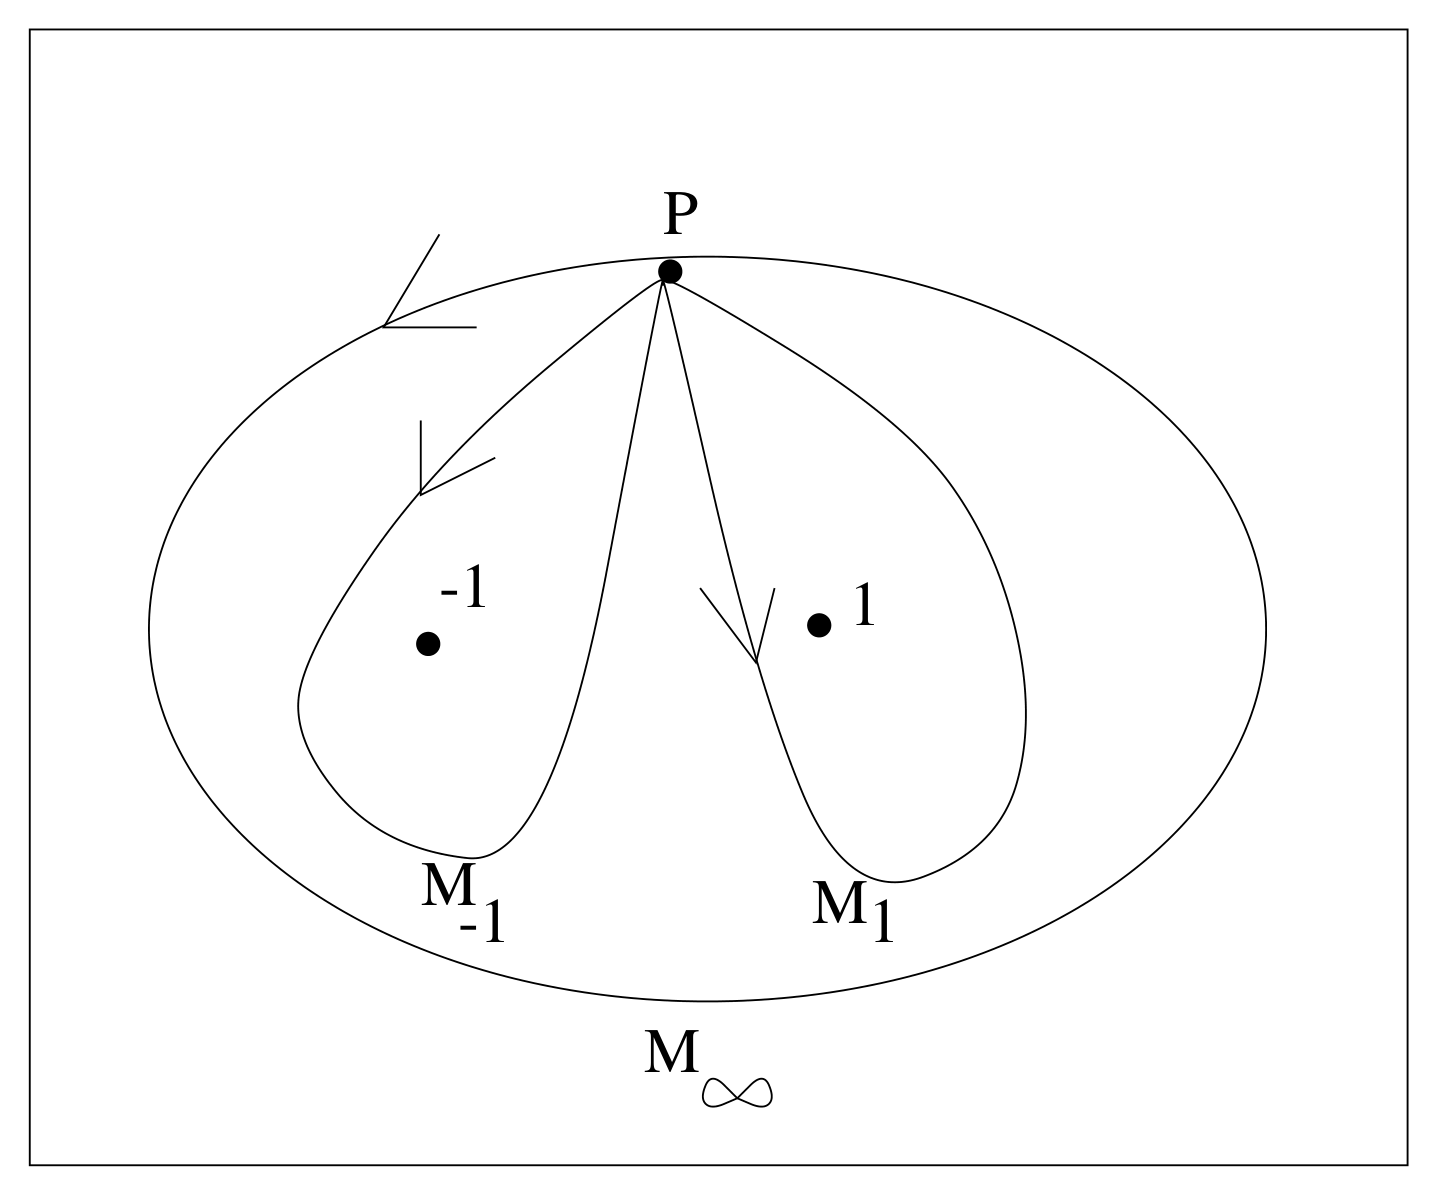
\includegraphics[width=0.64\textwidth]{figures/fig1_u_plane.png}
  \caption{$u$ 平面，以及绕 $1$、$-1$ 与 $\infty$ 的单值性。注意单值性定义中基点的
  选取。（原书 p.28）}
\end{figure}

% [Tutor Note: 图 1 特意画出基点 P，这一点很容易被忽略：三个单值矩阵都是"从 P 出发、绕对应奇点一圈再回到 P"所定义的，换基点相当于把三个矩阵同时共轭。§5.5 里 $u\to-u$ 会把基点挪到别处，所以 $M_\infty$ 的像 $M_\infty'=M_1'M_{-1}'=M_{-1}M_1$ 不能由 $M_\infty$ 直接共轭得到，尽管关系 $M_\infty=M_1M_{-1}$ 在变换后仍按同样顺序保持。印刷页 28（PDF 29）。]

矩阵 $M_{-1}$ 与 $M_1$ 共轭。事实上，若取
\begin{equation}
    A = T M_1 = \begin{pmatrix} -1 & 1 \\ -2 & 1 \end{pmatrix}, \tag{5.14}
\end{equation}
则
\begin{equation}
    M_{-1} = A M_1 A^{-1}. \tag{5.15}
\end{equation}

因此，$M_{-1}$ 可以像 $M_1$ 一样来自某个无质量粒子。对任意整数 $r$，把 $A$ 换成 $AM_1^r$ 后，(5.15) 仍然成立。

应当让哪一种粒子变成无质量，才能产生这个奇点？若把电荷排成行矢量 $q=(n_m,n_e)$，则产生单值性 $M$ 的无质量粒子满足 $qM=q$。例如，单值性 $M_1$ 来自荷矢量为 $q_1=(1,0)$ 的无质量磁单极子；利用 $M_1$ 的已知形式可直接验证 $q_1M_1=q_1$。对偶对称性意味着，这不仅对特定的单值性 $M_1$ 成立，而且对任何来自无质量粒子的单值性都成立。取 $q_{-1}=(1,-1)$，得到 $q_{-1}M_{-1}=q_{-1}$；因此单值性 $M_{-1}$ 来自荷为 $(1,-1)$ 的双荷子变为无质量。

看起来我们看到的是荷为 $(1,0)$ 或 $(1,-1)$ 的无质量粒子。然而，双荷子之间其实是完全平权的。半经典地存在的 BPS 饱和双荷子具有荷 $(1,n)$（或 $(-1,-n)$），其中 $n$ 为任意整数。无穷远处的单值性带来平移 $(1,n)\to(1,n-2)$。若在走到 $u=1$ 或 $u=-1$ 的奇点之前把这个平移做 $n$ 次，则产生这些奇点的无质量粒子将分别具有荷 $(1,-2n)$ 与 $(1,-1-2n)$。这相当于把基本群的表示用 $M_\infty^n$ 作共轭。

式 (5.14) 中那个特定的矩阵 $A$ 满足 $A^2=-1$；作为 $SL(2,\mathbb Z)$ 的自同构，$A^2=-1$ 等价于恒等映射。用 $A$ 作共轭实现了量子模空间底层的 $\mathbb Z_2$ 对称性；按我们的假设，这个对称性交换两个奇点。这个 $\mathbb Z_2$ 把 $M_1\mapsto M_1'=M_{-1}$、$M_{-1}\mapsto M_{-1}'=M_1$，以及 $M_\infty\mapsto M_\infty'=M_1'M_{-1}'=M_{-1}M_1$。注意 $M_\infty'$ 并不只是由 $M_\infty$ 共轭得到的，而是（在变换下）关系 $M_\infty=M_1M_{-1}$ 仍被保持。原因在于：单值性的定义需要选择基点（只要考虑流形的基本群在非阿贝尔群中的表示，就都会如此），如图 1 所示。操作 $u\to -u$ 会作用到基点上，因此在确定 $M_\infty$ 于 $\mathbb Z_2$ 下如何变换时，必须把这一点考虑进去。

还可以进一步证明：若假定 $M_1$ 与 $M_{-1}$ 之间存在 $\mathbb Z_2$ 对称性，则它们必须与 $T^2$ 共轭，而不能与 $T$ 的其他幂共轭。在我们推导单值性 (5.12) 时，其中的 2 来自与 $\mathbb Z_2$ 对称性假设完全无关的东西，即半经典地存在的磁单极子的电荷与重数。

\subsection{磁单极子凝聚与禁闭}

现在我们来解释一个相当令人满意的物理现象；事实上，当初这些结果中的一部分被发现时，它正处于核心位置。

回忆一下：底层的 $\mathcal N=2$ 手征多重态 $\mathcal A$ 在 $\mathcal N=1$ 超对称下分解为一个矢量多重态 $W_\alpha$ 和一个手征多重态 $\Phi$。把 $\mathcal N=2$ 破缺到 $\mathcal N=1$ 时，可以为这个手征多重态加上超势 $W=m\,\mathrm{Tr}\,\Phi^2$。这给 $\Phi$ 一个裸质量，使低能理论化为纯 $\mathcal N=1$ 规范理论。低能理论具有 $\mathbb Z_4$ 手征对称性。人们强烈相信这个理论会产生质量间隙，并伴随电荷禁闭以及 $\mathbb Z_4$ 自发破缺到 $\mathbb Z_2$。此外，除了这种对称性破缺所造成的简并之外没有真空简并，因此恰有两个真空态 [32]。

这一现象如何在低能有效 $\mathcal N=2$ 理论中重现？那个理论有量子真空的模空间 $\mathcal M$。至少在半经典意义上，无质量谱只由未破缺的 $U(1)$（$SU(2)$ 的子群）的那个阿贝尔手征多重态 $\mathcal A$ 组成。

如果这些确实是唯一的无质量粒子，那么打开 $m$ 在低能理论中的效应可以如下分析。算符 $\mathrm{Tr}\,\Phi^2$ 在低能理论中由一个手征超场 $U$ 表示。它的第一个分量是标量场 $u$，其期望值为
\begin{equation}
    \langle u\rangle = \langle \mathrm{Tr}\,\phi^2\rangle \tag{5.16}
\end{equation}
（$\phi$ 是超场 $\Phi$ 的 $\theta=0$ 分量。）这是模空间上的全纯函数。至少对小 $m$，我们应在低能拉格朗日量中加入有效超势 $W_{\mathrm{eff}}=mU$（稍后我们会证明，对大的 $m$ 它也是精确表达式）。

打开超势 $mU$ 也许会把几乎所有的真空都消掉，并在残存的真空中给 $\mathcal A$ 的标量分量以质量。但如果讨论中没有额外的自由度，$\mathcal A$ 中的规范场仍会是无质量的。要让规范场获得质量（这是必需的，因为当 $m\neq 0$ 时微观理论有质量间隙），需要以下两者之一：(i) 额外的轻规范场，从而得到非阿贝尔规范理论和可能的强耦合效应；(ii) 轻的带荷场，从而可能实现希格斯机制。

于是我们得知（正如讨论单值性时那样）：在 $\mathcal M$ 的某处必定出现额外的无质量态。由于前面已经讨论过的原因，方案 (i) 看来没有吸引力。我们转而考虑方案 (ii)，并附加一个来自先前讨论的条件：所涉及的轻带荷场是磁单极子和双荷子。

在存在无质量磁单极子的点附近，只要用原光子的对偶场 $\mathcal A_D$ 来描述规范场，磁单极子就可以用 $\mathcal N=1$ 语言下的普通（局域）手征超场 $M$ 与 $\widetilde M$ 表示。超势为
\begin{equation}
    \widehat W = \sqrt{2}\,\mathcal A_D M\widetilde M + m\,U(\mathcal A_D), \tag{5.17}
\end{equation}
其中第一项是 $m=0$ 理论的 $\mathcal N=2$ 不变性所要求的，第二项是微观扰动 $m\,\mathrm{Tr}\,\Phi^2$ 诱导出的对有效超势的贡献。
% [Tutor Note: (5.17) 的形式由电荷决定：$m$ 带荷 $2$，$M$ 与 $\widetilde M$ 各带荷 $1$，所以超势中 $m$ 的一次项要乘一个带荷 $2$ 的 $\mathcal A_D$ 的函数，$M\widetilde M$ 项也要带荷 $2$；第一项则由 $m=0$ 时的 $\mathcal N=2$ 不变性所要求。所谓"精确"，指非重整化定理排除了 $m$ 的高阶修正。印刷页 30（PDF 31）。]

超势 (5.17) 是精确的，这一点可按如下方式用 [1] 的非重整化定理建立。当 $m=0$ 时，理论具有 $SU(2)_R$ 不变性。只需考虑它的 $U(1)_J$ 子群，即式 (2.2)。这是一个 $\mathcal N=1$ 的 $R$ 对称性，在此对称性下 $\Phi$ 的荷为零。两个 $\mathcal N=1$ 手征场 $M$ 与 $\widetilde M$ 处于同一个 $\mathcal N=2$ 超多重态中。因此按式 (2.4)，它们都带荷 1。微观超势中出现 $m\,\mathrm{Tr}\,\Phi^2$ 这一项，说明参数 $m$ 带荷 2。低能超势 $\widehat W(m,M\widetilde M,\mathcal A_D)$ 是其变量的全纯函数，并且在 $U(1)_J$ 下应带荷 2。要求它在 $m=M\widetilde M=0$ 处正则，可得其形式为 $\widehat W=m f_1(\mathcal A_D)+M\widetilde M f_2(\mathcal A_D)$。函数 $f_1$ 与 $f_2$ 与 $m$ 无关，可通过考察小 $m$ 极限定出，结果便得到 (5.17)。

低能真空结构容易分析。真空态（在规范变换意义下）对应于满足附加条件 (5.19) 的 (5.18) 的解：
\begin{equation}
    \mathrm{d}\widehat W = 0 \tag{5.18}
\end{equation}
\begin{equation}
    |M| = |\widetilde M| \tag{5.19}
\end{equation}
（我们用 $M$ 与 $\widetilde M$ 同时表示超场及其第一个分量）。后一条件来自 $D$ 项为零。把这些条件实现出来：当 $m=0$ 时，真空态对应 $M=\widetilde M=0$、$a_D$ 任意；这恰是我们熟悉的模空间 $\mathcal M$。当 $m\neq 0$ 时结果大不相同。此时得到
\begin{equation}
\begin{gathered}
    \sqrt{2}M\widetilde M + m\frac{\mathrm{d}u}{\mathrm{d}a_D} = 0\\
    a_D M = a_D\widetilde M = 0.
\end{gathered}
\tag{5.20}
\end{equation}
假定 $\mathrm{d}u\neq 0$，第一个方程要求 $M,\widetilde M\neq 0$，于是第二个方程要求 $a_D=0$。再施加条件 (5.19)，便得到在规范变换意义下唯一的解：
\begin{equation}
    M = \widetilde M = \left(-m u'(0)/\sqrt{2}\right)^{1/2}. \tag{5.21}
\end{equation}

在这个真空附近展开，容易看出存在质量间隙。例如，由于 $M,\widetilde M\neq 0$，规范场通过希格斯机制获得质量。这里发生的是磁的希格斯机制，因为取得期望值的场正是磁单极子！磁单极子的凝聚将导致电荷禁闭。这样，我们就从低能有效作用量的角度解释了：为什么加上 $m\,\mathrm{Tr}\,\Phi^2$ 超势后，微观理论会变得禁闭。

我们还注意到，在扰动超势存在时，微观理论具有 $\mathbb Z_4$ 整体对称性，它自发破缺到 $\mathbb Z_2$。这种破缺在有效理论中表现得很清楚：破缺的对称性把 $a_D=0$、存在无质量磁单极子的那个点，与 $a-a_D=0$、存在无质量双荷子的那个点互换。因此，有效理论从这两个额外无质量粒子的点（它们对应上面讨论过的 $u$ 平面上的两个奇点）得到两个真空态，两者由被破缺的对称性相联系；这与微观上的预期一致。

在微观描述中，人们把（$m\neq 0$ 时）两个真空态的这些性质归因于难以理解的强规范耦合。而在低能理论中，我们得到了一个非常平和的描述：它是磁单极子与光子的弱耦合理论；当 $m=0$ 时，耦合常数在红外流向零；一般地，它流向 $-1/\ln m$ 量级的值，因为这就是弱耦合 QED 的行为。原来的电规范耦合是磁耦合的倒数，因此在红外流向 $-\ln m$ 量级的值；在这个意义上，当 $m$ 很小且非零时残存的两个真空是强耦合的。

有效超势 (5.17) 对磁单极子变轻的 $u_0$ 点附近的低能物理给出了良好的描述。它在远离 $u_0$ 处的含义是什么？在那里，除了磁单极子的期望值及其质量之外，它们的性质几乎没有一项能从有效拉格朗日量正确推断出来。若试图把它解析延拓到 $u=-u_0$（那里应当出现无质量双荷子），有效拉格朗日量会遇到更大的困难。不可能存在一个同时把磁单极子和双荷子都当作基本场的有效场论，因为它们不是相对定域的。我们讨论的这个理论是一个有趣的例子：在任何一个真空的邻域内，都有良好的低能有效理论描述；但不存在一个处处合理的低能有效理论。

\subsection{有效参数}

最后，我们来收束一些遗留的问题，同时为下一节给出模型的解做准备。

上面我们在假定 $\mathrm{d}u\neq 0$ 的前提下，对 $m\neq 0$ 找到了两个真空态。在任何 $\mathrm{d}u=0$ 的点，我们都会得到额外的态（其 $M=\widetilde M=0$）。微观理论中正确的真空数目是 2，我们不希望有额外的真空态，因此假定 $\mathrm{d}u\neq 0$ 处处成立。
% [Tutor Note: 这里的 $\mathrm{d}u$ 与 (5.20) 中的 $\mathrm{d}u/\mathrm{d}a_D$ 都指 $u$ 作为 $a_D$ 的函数之导数，不是微分形式；$\mathrm{d}u=0$ 指该导数为零（临界点），此时会多出 $M=\widetilde M=0$、$a_D$ 任意的真空。把 $\mathrm{d}u\neq0$ 假定成"处处成立"是为了让真空数恰好为 2，这是 §6 提出解时的前提之一，并非已证明的结论；(5.21) 中被开方的 $-m u'(0)$ 也须为正，才能得到实的 $M$。印刷页 31–33（PDF 32–34）。]

$\mathrm{d}u\neq 0$ 意味着 $u$ 在真空空间上处处是良好的局部坐标。它是否也是良好的整体坐标？问题在于：给定 $u$ 是否恰好有一个真空。由式 (5.16)，$u$ 就是 $\mathrm{Tr}\,\phi^2$ 的期望值，把它看作真空空间上的函数。至少当 $u=\mathrm{Tr}\,\phi^2$ 很大时，微扰论可靠，给定 $u$ 恰好有一个真空。这些事实合在一起强烈提示：$u$ 是真空空间 $\mathcal M$ 上良好的整体坐标。

在下一节提出模型的解时，我们将假定 $\mathcal M$ 就是 $u$ 平面（其中 $u$ 等于 $\mathrm{Tr}\,\phi^2$ 的期望值），并恰有我们上面提出的那两个奇点。我们将选取一种重整化约定，使 $u$ 平面上的奇点位于 $1$ 和 $-1$。利用下一节将要提出的模型的解，就可以与微扰论比较，并确定这种约定与其他约定（例如 $\overline{MS}$）相比如何。


% ===== 片段：sections/s06.tex =====

\section{模型的解}
\begin{keypoints}
  \item \textbf{出发点：} 量子真空的模空间 $\Mm$ 取为 $u$ 平面，奇点在 $u=1,-1,\infty$；在挖去这三点的
        $u$ 平面上有一个平坦的 $SL(2,\Z)$ 丛 $V$，$(a_D,a)$ 是它的全纯截面。
  \item \textbf{输入：} 单值矩阵 (6.1) 加上三个奇点附近的渐近行为 (6.2)(6.3)，再要求度规正定，
        即 $\Im\tau>0$（见式 (6.4)(6.5)）——这些条件合起来唯一确定了这个截面。
  \item \textbf{关键技巧：} 用椭圆曲线族 $E_u$：$y^2=(x-1)(x+1)(x-u)$ 的周期来构造截面；
        只要取 $\dd\lambda/\dd u=f(u)\lambda_1$，就自动有 $\tau=\tau_u$，从而 $\Im\tau>0$，
        而唯一可行的 $f$ 是 $-\sqrt2/4\pi$。
  \item \textbf{显式结果：} $\lambda$ 在一维闭链上的周期积分 (6.22)(6.23) 给出 $a,a_D$；
        在 $u=\infty,1$ 处逐一验证渐近行为 (6.24)--(6.30)，复现出单值性 $a\to a-2a_D$。
  \item \textbf{谱：} BPS 谱不必在 $\Gamma(2)$ 下不变，因为穿过 $a_D/a$ 为实的曲线时谱可以跳变；
        在实 $u$ 轴上 $|u|>1$ 处可证明 $a_D/a$ 非实，故从半经典区走向 $u=\pm1$ 不会越过跳跃曲线，
        奇点所需的磁单极子与双荷子必须在半经典区存在。
\end{keypoints}

本节我们终于要把各部分拼在一起，再加上几个新要素，提出关于模型之解的方案。

量子真空的模空间 $\Mm$ 应当就是 $u$ 平面：奇点位于 $1$、$-1$ 与 $\infty$，另有一个按
$u\leftrightarrow-u$ 作用的 $\Z_2$ 对称性。对偶意味着：在挖去这三点的 $u$ 平面上存在一个
平坦的 $SL(2,\Z)$ 丛 $V$，它绕 $\infty$、$1$ 与 $-1$ 的单值性如下：
\begin{align}
  M_\infty&=\begin{pmatrix}-1&2\\[1pt]0&-1\end{pmatrix}\notag\\
  M_1&=\begin{pmatrix}1&0\\[1pt]-2&1\end{pmatrix} \tag{6.1}\\
  M_{-1}&=\begin{pmatrix}-1&2\\[1pt]-2&3\end{pmatrix}.\notag
\end{align}

量 $(a_D(u),a(u))$ 是丛 $V$ 的全纯截面（严格说，是 $V\otimes\C$ 的全纯截面）。这个截面由它的
渐近行为确定。在 $u=\infty$ 附近，
\begin{align}
  a&\approx\sqrt{2u}\notag\\
  a_D&\approx i\,\frac{\sqrt{2u}}{\pi}\ln u. \tag{6.2}
\end{align}
% [Tutor Note: 单值矩阵 (6.1) 与渐近式 (6.2)(6.3) 合起来就是确定全纯截面 $(a_D,a)$ 的全部
% 边界数据——本质上是一个黎曼--希尔伯特问题：给定奇点处的单值性与无穷远处的行为，
% 全纯截面对数唯一。这正是“对偶唯一确定低能理论”的技术含义。]
在 $u=1$ 附近，
\begin{align}
  a_D&\approx c_0(u-1)\notag\\
  a&\approx a_0+\frac{i}{\pi}a_D\ln a_D, \tag{6.3}
\end{align}
其中 $a_0,c_0$ 是常数。$u=-1$ 附近的行为类似，只需把 $a_D$ 换成 $a-a_D$。
% [Tutor Note: 把 $a_D$ 换成 $a-a_D$ 不是随手改写（(6.3) 中的 $u-1$ 相应地理解为 $u+1$）。
% 由 (6.1)，$M_{-1}$ 把
% $a_D\to-a_D+2a$、$a\to-2a_D+3a$，故组合 $a-a_D$ 在单值性下不变，而
% $a\to a+2(a-a_D)$。所以 $u=-1$ 处变轻的正是 $a-a_D\propto(u+1)$，
% 对应荷 $(n_m,n_e)=(1,-1)$ 的双荷子。]

此外还有一个重要的约束。$u$ 平面上的度规可以写成
\begin{equation}
  (\dd s)^2=\Im(\tau)\cdot|\dd a|^2 \tag{6.4}
\end{equation}
其中
\begin{equation}
  \tau=\frac{\dd a_D/\dd u}{\dd a/\dd u}. \tag{6.5}
\end{equation}

为保证度规正定，$\Im(\tau)$ 必须正定。我们无需另行指定 $\tau$ 在 $-1$、$1$、$\infty$ 附近的
渐近行为，因为它由 $a$ 与 $a_D$ 的渐近行为决定。
% [Tutor Note: (6.4)(6.5) 中的 $\tau$ 就是预势的二阶导数：由 $a_D=\partial\Ff/\partial a$
% 得 $\tau=\partial^2\Ff/\partial a^2$，而 (6.5) 只是链式法则。$\Im\tau=4\pi/g^2>0$ 是弱耦合
% 区的要求；让它在整个模空间上成立，正是下面用来挑选 $\lambda$ 的原则。]

这些条件之所以能实际求解，关键在于这个平坦的 $SL(2,\Z)$ 丛有一个很好的解释。首先注意，
式 (6.1) 中的单值矩阵全都模 2 同余于 1。因此它们生成不了整个 $SL(2,\Z)$——最多只能生成
$SL(2,\Z)$ 中由模 2 同余于 1 的矩阵组成的子群。这个子群通常叫作 $\Gamma(2)$。事实上，
$M_\infty$ 与 $M_1$ 确实生成 $\Gamma(2)$。\footnote{本段中这一断言及其他断言的简捷证明，
见 [33] 第 92--93 页。} 再者，挖去 $1$、$-1$ 与 $\infty$ 的 $u$ 平面还有一个非常特殊的解释。

它可以看成上半平面 $H$ 模去 $\Gamma(2)$ 得到的商。的确，$\Gamma(2)$ 在 $SL(2,\Z)$ 中的指数为 6，
所以商 $H/\Gamma(2)$ 是通常模域的六重覆盖。这个商有三个尖点，可以取在 $1$、$-1$ 与
$\infty$，其单值性恰好是 (6.1) 中的那些。
% [Tutor Note: 把 $u$ 平面等同于 $H/\Gamma(2)$ 是本节的结构性一步（原书 pp. 34--35）。
% $\Gamma(2)$ 指数为 6，故 $H/\Gamma(2)$ 是模域的六重覆盖；三个尖点 $\infty,1,-1$
% 与 (6.1) 的三个单值性一一对应，这是后面把曲线族写成 (6.6) 的依据。]

以 $H/\Gamma(2)$ 为参数空间的曲线族可以写得很具体，其方程为
\begin{equation}
  y^2=(x-1)(x+1)(x-u). \tag{6.6}
\end{equation}

这里的想法是：对每个 $u$，式 (6.6) 确定一个亏格一的黎曼面 $E_u$。这个方程描述 $x$ 平面的一个
二重覆盖，分支点在 $-1$、$1$、$\infty$ 与 $u$。当（且仅当）两个分支点重合时，曲线 $E_u$ 变
奇异。这恰好发生在 $u=1$、$-1$ 或 $\infty$。

顺便注意，(6.6) 有一个明显的对称性 $w$：$u\to-u$、$x\to-x$、$y\to\pm iy$。它生成一个
$\Z_4$ 对称性，但作用在 $u$ 平面上只是它的一个 $\Z_2$ 商。事实上，$P=w^2$ 在 $u$ 与 $x$ 上的
作用平凡，只把 $y$ 映为 $-y$。后面会看到，$a$ 与 $a_D$ 在 $y\to-y$ 下为奇，因而在 $P$ 下也
为奇。刚刚描述的对称结构，正是我们要解的场论所具有的对称结构。

黎曼面 $E_u$ 有二维的第一同调群 $V_u=H^1(E_u,\C)$。这些 $V_u$ 是挖去若干点的 $u$ 平面上某个
平坦丛 $V$ 的纤维，而 $(a_D,a)$ 正是这个丛的一个截面。正如我们将看到的，这是描述该丛的
方便方式。
% [Tutor Note: 原文把 $V_u=H^1(E_u,\C)$ 称为“第一同调群”，而 $H^1$ 通常是上同调。
% 此处两者通过周期配对互为对偶，把 $V_u$ 看成 de Rham（上）同调并无矛盾；原书第 36 页
% 紧接着用 Hodge 分解 $H^1=H^{1,0}\oplus H^{0,1}$，也印证了这一点。]

丛 $V$ 可以局部平凡化：在 $E_u$ 上取一对独立且连续变化的一维闭链（one-cycle）
$\gamma_1,\gamma_2$ 即可；它们可以归一化，使相交数为
\begin{equation}
  \gamma_1\cdot\gamma_2=1. \tag{6.7}
\end{equation}

空间 $H^1(E_u,\C)$ 可以看成 $E_u$ 上留数为零的亚纯 $(1,0)$-形式，模去恰当形式（或全导数）
所得的空间。启发式的想法是：若 $\lambda$ 是这样的一形式，则它代表 $H^1(E_u,\C)$ 中的一个
元素，因为它可以与一维闭链配对，方式为
\begin{equation}
  \gamma\to\oint_\gamma\lambda. \tag{6.8}
\end{equation}

$\lambda$ 的留数为零这一条件，保证该配对在 $\gamma$ 形变时不变，即使形变跨过 $\lambda$ 的
极点也如此。人们把 $\lambda$ 与 $\lambda+\dd w$ 等同起来（其中 $w$ 是亚纯函数），因为恰当
微分 $\dd w$ 对围道积分 (6.8) 没有贡献。

$H^1(E_u,\C)$ 是二维的，任意两个线性无关的元素都构成一组基，例如
\begin{equation}
  \lambda_1=\frac{\dd x}{y}\quad\text{and}\quad \lambda_2=\frac{x\,\dd x}{y}. \tag{6.9}
\end{equation}

这里 $\lambda_1$ 实际上是全纯微分，连无穷远处也没有极点；不计标量倍数，它是 $E_u$ 上唯一的
全纯微分。（按 $H^1(E_u,\C)$ 的 Hodge 分解，它代表 $H^{1,0}$ 中的一个元素。）若在 $E_u$ 上取
一组按 (6.7) 归一化的一维闭链，则周期
\begin{equation}
  b_i=\oint_{\gamma_i}\lambda_1,\qquad i=1,2 \tag{6.10}
\end{equation}
满足
\begin{equation}
  \frac{b_1}{b_2}=\tau_u, \tag{6.11}
\end{equation}
其中 $\tau_u$ 是椭圆曲线 $E_u$ 的通常 $\tau$ 参数，它具有基本性质
\begin{equation}
  \Im(\tau_u)>0. \tag{6.12}
\end{equation}

换一组 $\gamma$ 基时，$\tau_u$ 按 $SL(2,\Z)$ 在上半平面上的标准作用变换。至于 $\lambda_2$，
它唯一的极点是无穷远处的二阶极点；那里的留数为零，因为亚纯微分的留数之和无论如何都为零。

既然 (6.9) 给出 $H^1(E_u,\C)$ 的一组基，平坦丛 $V_u$ 的任意截面都可以写成
\begin{equation}
  \lambda=a_1(u)\lambda_1+a_2(u)\lambda_2. \tag{6.13}
\end{equation}

这种表示未必方便，因为有时更方便的是利用加上某个函数 $w$ 的 $\dd w$ 的自由度。无论如何，
选定截面 $\lambda$ 之后，要提取它的分量 $a_D$ 与 $a$，只需取一维闭链基 $\gamma_1,\gamma_2$，
并定义
\begin{align}
  a_D&=\oint_{\gamma_1}\lambda\notag\\
  a&=\oint_{\gamma_2}\lambda. \tag{6.14}
\end{align}
若换一组 $\gamma_i$，$(a_D,a)$ 就按 $SL(2,\Z)$ 的某个元素变换。

现在我们要加一个条件：由 (6.5) 定义的 $\tau$ 满足 $\Im(\tau)>0$。有一个显然的办法可以满足
它。注意到
\begin{align}
  \frac{\dd a_D}{\dd u}&=\oint_{\gamma_1}\frac{\dd\lambda}{\dd u}\notag\\
  \frac{\dd a}{\dd u}&=\oint_{\gamma_2}\frac{\dd\lambda}{\dd u}. \tag{6.15}
\end{align}
假设
\begin{equation}
  \frac{\dd\lambda}{\dd u}=f(u)\lambda_1=f(u)\frac{\dd x}{y} \tag{6.16}
\end{equation}
其中 $f(u)$ 只是 $u$ 的函数。于是得到
\begin{align}
  \frac{\dd a_D}{\dd u}&=f(u)b_1\notag\\
  \frac{\dd a}{\dd u}&=f(u)b_2, \tag{6.17}
\end{align}
其中 $b_i$ 按 (6.10) 定义。因此
\begin{equation}
  \tau=\frac{\dd a_D/\dd u}{\dd a/\dd u}=\frac{b_1}{b_2}=\tau_u, \tag{6.18}
\end{equation}
从而 $\Im(\tau)>0$。

反之，若处处 $\Im(\tau)>0$，则 $\tau=\tau_u$，且 $\lambda$ 如上。要看出这一点，先注意：若
处处 $\Im(\tau)>0$，则对每个 $u$，$\tau(u)$ 都是某条椭圆曲线的 $\tau$ 参数。此外，
$(\dd a_D/\dd u,\dd a/\dd u)$ 在 $SL(2,\Z)$ 下的变换方式与 $(a_D,a)$ 相同，因此给出同一个
平坦丛的截面。于是，由 $u\to\tau(u)$ 确定的曲线族与由 $u\to\tau_u$ 确定的曲线族 $E_u$ 具有
相同的单值性（与奇点）。由一般理由可知，这两个族重合。
% [Tutor Note: (6.16) 要求 $\dd\lambda/\dd u$ 正比于只依赖 $u$ 的 $\lambda_1$，这是保证
% $\tau=\tau_u$ 的关键：$b_1/b_2=\tau_u$ 是椭圆曲线的模，于是 (6.18) 自动给出 $\Im\tau>0$，
% 无需另外求解。$f$ 必须是常数，否则 $\dd\lambda$ 会在某处引入多余的极点或零点；
% (6.19) 显示 $f=-\sqrt2/4\pi$ 恰好可行。]

剩下的任务是选定 $f$，并验证 $a_D$ 与 $a$ 在 $u=1$、$-1$、$\infty$ 附近具有所要求的渐近
行为。我们实际上会证明：取 $f=-\sqrt2/4\pi$ 时一切都对。届时也就清楚，这是唯一可行的选择；
特别地，非常数的 $f$ 会在某处引入多余的极点或零点。

首先，给定 (6.16) 之后，找 $\lambda$ 并不困难。可取
\begin{equation}
  \lambda=\frac{\sqrt2}{2\pi}\,\frac{\dd x\,\sqrt{x-u}}{\sqrt{x^2-1}}
        =\frac{\sqrt2}{2\pi}\,\frac{\dd x\,y}{x^2-1}. \tag{6.19}
\end{equation}

显然，这个表达式对 $u$ 求导就复现出 (6.16)，其中 $f=-\sqrt2/4\pi$。$\lambda$ 的留数为零，
因为
\begin{equation}
  \lambda=\frac{\sqrt2\,(\lambda_2-u\lambda_1)}{2\pi} \tag{6.20}
\end{equation}
其中 $\lambda_i$ 如上。由 (6.19) 第二式可以看出，$\lambda$ 在 $P=w^2$ 下为奇；正因如此，按
上面给出的定义，$P$ 会把 $a$ 与 $a_D$ 的符号反转。

\begin{figure}[htbp]
  \centering
  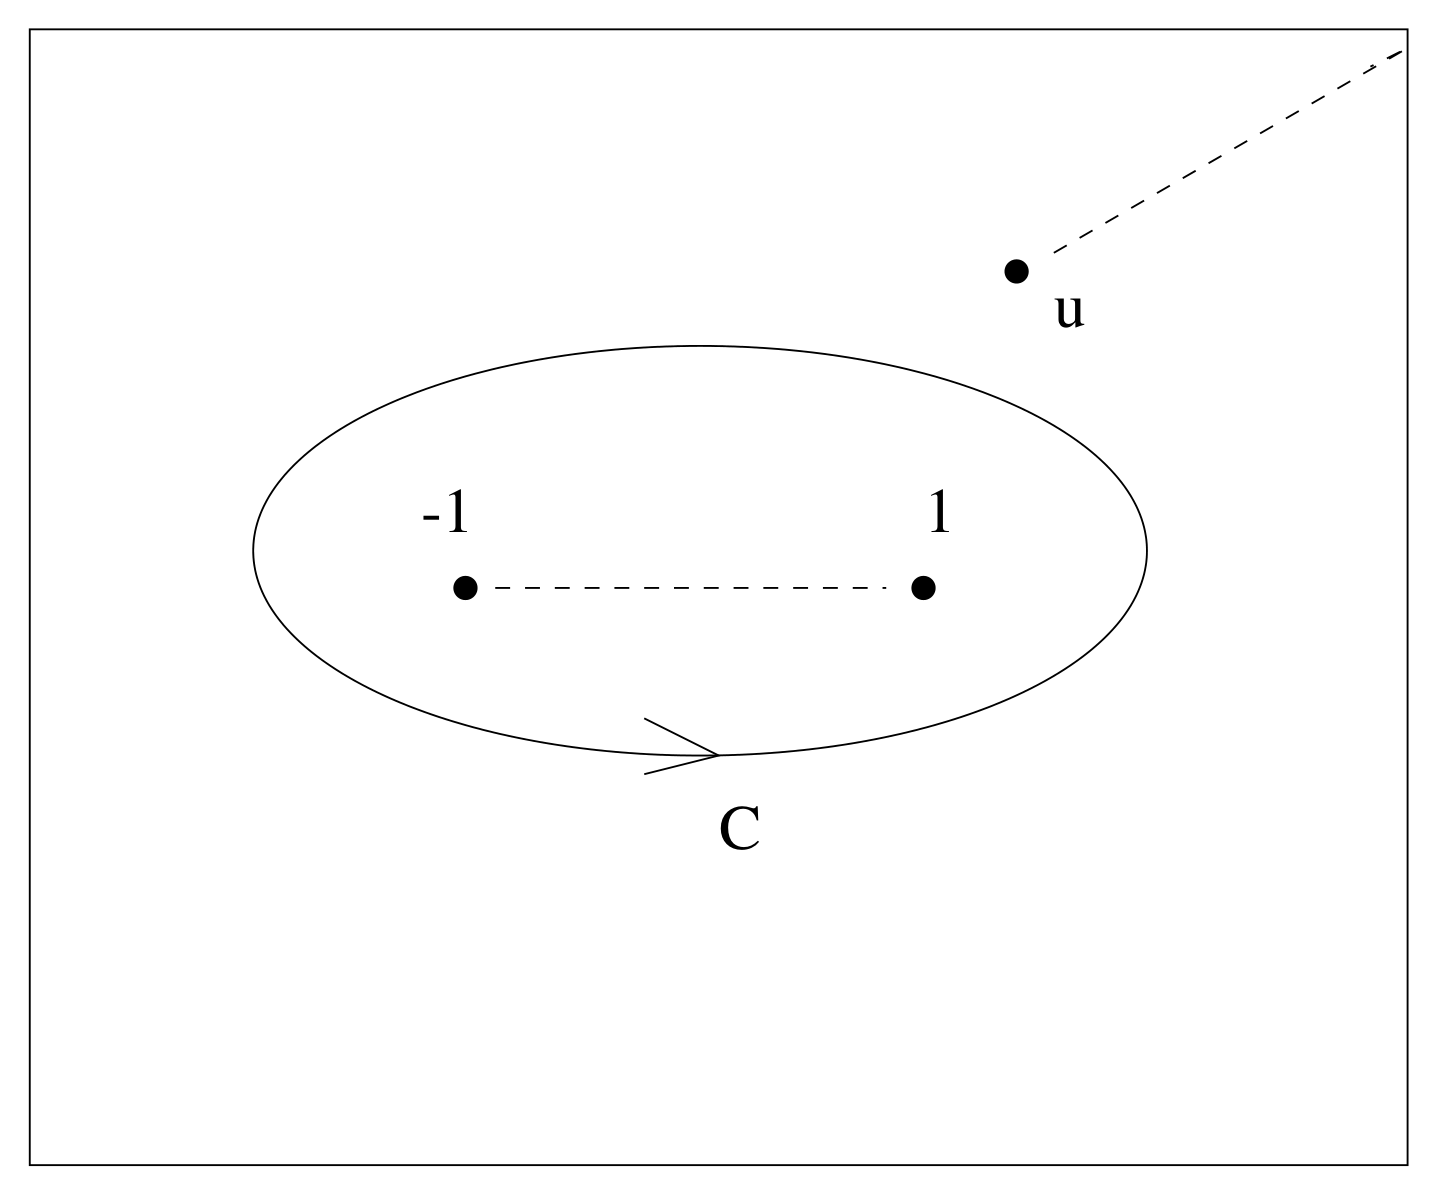
\includegraphics[width=0.64\textwidth]{figures/fig2_one_cycle.png}
  \caption{$E_u$ 上的一个非平凡一维闭链，来自 $x$ 平面中绕两个分支点的围道。
  图中虚线标出 $x$ 平面上的割线。（原书 p.38）}
\end{figure}
% [Tutor Note: 图 2 属于此处（原书 p.38）：$x$ 平面中的圆周 $C$ 绕两个分支点，提升到 $E_u$
% 上就是非平凡闭链 $\gamma$。图中的虚线表示割线、实线表示闭链；这张图是理解 (6.21) 中
% 因子 2 与 (6.22)(6.23) 积分限的直接依据。]

现在我们需要 $E_u$ 上一维闭链的显式基。这些闭链可以这样构造：$x$ 平面中绕两个分支点的
圆周 $C$，提升为 $E_u$ 上的一条非平凡闭链 $\gamma$。（撇开任何拓扑论证，这条闭链的非平凡性
也可以由我们将要写出的积分不为零看出。）例如，如图 2 所示，取 $C$ 绕 $x=1$ 与 $x=-1$ 处的
分支点一圈。我们要积分的微分形式 $\lambda$，按 (6.19) 第一式看作 $x$ 平面上的形式，带有因子
$\sqrt{(x-u)/(x^2-1)}$，因此需要分支割线。可以取割线从 $-1$ 到 $1$、并从 $u$ 到 $\infty$，
如图 2 所示。

然后可以把 $C$ 形变到只绕 $-1$ 与 $1$ 之间的割线一圈。于是
\begin{equation}
  \oint_\gamma\lambda=\frac{\sqrt2}{2\pi}\oint_C\frac{\dd x\,\sqrt{x-u}}{\sqrt{x^2-1}}
  =\frac{\sqrt2}{\pi}\int_{-1}^{1}\frac{\dd x\,\sqrt{x-u}}{\sqrt{x^2-1}}. \tag{6.21}
\end{equation}
最后一步出现因子 2，是因为沿 $C$ 的积分包含一段从 $-1$ 到 $1$ 的积分，再加上割线另一侧
从 $1$ 回到 $-1$ 的积分；这两段的贡献相等。

现在可以落实 (6.14) 中 $a$ 与 $a_D$ 的定义。把刚描述的围道取作 $\gamma_2$，就有
\begin{equation}
  a=\frac{\sqrt2}{\pi}\int_{-1}^{1}\frac{\dd x\,\sqrt{x-u}}{\sqrt{x^2-1}}. \tag{6.22}
\end{equation}
类似地，用绕 $1$ 与 $u$ 处分支点的圆周来定义另一条闭链 $\gamma_1$，则可取
\begin{equation}
  a_D=\frac{\sqrt2}{\pi}\int_{1}^{u}\frac{\dd x\,\sqrt{x-u}}{\sqrt{x^2-1}}. \tag{6.23}
\end{equation}

当然，选取这组特殊的一维闭链，是为了在 $u$ 平面的奇点附近得到所需的行为。平方根的出现
意味着 $a$ 与 $a_D$ 的整体符号没有定义。这与下面的事实一致：从一开始，经典关系 $a^2=2u$
就说明，由规范不变量 $u$ 只能把 $a$ 确定到相差一个符号。
% [Tutor Note: (6.21)--(6.23) 的积分限与符号依赖于割线和平方根分支的取法；这正是
% “$a$ 与 $a_D$ 的整体符号没有定义”的含义，也与经典关系 $a^2=2u$ 相容。取 $\gamma_2$ 绕
% $-1,1$、$\gamma_1$ 绕 $1,u$，是为了在 $u\to\infty$ 时让 $a$ 呈 $\sqrt{2u}$、在 $u\to1$ 时
% 让 $a_D$ 变轻。]

只需研究 $a$ 与 $a_D$ 在 $u=\infty$ 与 $u=1$ 附近的行为，因为 $u=-1$ 附近的行为由前面描述
的 $u$ 平面的 $\Z_2$ 对称性决定。

在 $u=\infty$ 附近，得到
\begin{equation}
  a\approx\frac{\sqrt{2u}}{\pi}\int_{-1}^{1}\frac{\dd x}{\sqrt{1-x^2}}=\sqrt{2u} \tag{6.24}
\end{equation}
以及（作变量代换 $x=uz$ 之后）
\begin{equation}
  a_D=\frac{\sqrt{2u}}{\pi}\int_{1/u}^{1}\frac{\dd z\,\sqrt{z-1}}{\sqrt{z^2-u^{-2}}}. \tag{6.25}
\end{equation}
当 $u\to\infty$ 时，该积分在 $z=0$ 附近出现对数发散；取出这个发散项，得到
\begin{equation}
  a_D\approx i\,\frac{\sqrt{2u}\,\ln u}{\pi}. \tag{6.26}
\end{equation}

当然，这个对数正是大 $u$ 的半经典区中渐近自由的标志。

$u=1$ 附近的行为同样容易确定。由 (6.25) 得到
\begin{align}
  a_D&=\frac{\sqrt{2u}}{\pi}\int_{1/u}^{1}
       \frac{\dd z\,\sqrt{z-1}}{\sqrt{z+u^{-1}}\,\sqrt{z-u^{-1}}}
       \approx\frac{1}{\pi}\int_{1/u}^{1}\frac{\dd z\,\sqrt{z-1}}{\sqrt{z-u^{-1}}}\notag\\
      &=\frac{i}{2}\left(1-\frac{1}{u}\right)\approx\frac{i\,(u-1)}{2}. \tag{6.27}
\end{align}

那么 $a$ 呢？在 $u=1$ 处，$a$ 的积分为
\begin{equation}
  a(u=1)=\frac{\sqrt2}{\pi}\int_{-1}^{1}\frac{\dd x}{\sqrt{x+1}}=\frac{4}{\pi}. \tag{6.28}
\end{equation}
然而，$a$ 对 $u$ 的导数由一个积分给出，
\begin{equation}
  \frac{\dd a}{\dd u}=-\frac{\sqrt2}{2\pi}\int_{-1}^{1}
  \frac{\dd x}{\sqrt{(x+1)(x-1)(x-u)}} \tag{6.29}
\end{equation}
当 $u\to1$ 时，它在 $x=1$ 附近对数发散。取出对数的系数，就得到 $a$ 的展开式
\begin{equation}
  a=\frac{4}{\pi}-\frac{(u-1)\ln(u-1)}{2\pi}+\ldots \tag{6.30}
\end{equation}
比较 (6.30) 与 (6.27)，便得到 $u=1$ 附近所要的单值性 $a\to a-2a_D$。
% [Tutor Note: (6.27) 中间一步用到了 $\sqrt{2u}/\sqrt{z+u^{-1}}\approx1$
% （$u\approx1$，$z\in[1/u,1]$）；右端的 $i$ 来自分支选择：在该区间上
% $\sqrt{z-1}=i\sqrt{1-z}$，于是积分给出 $\frac{i}{2}\left(1-\frac1u\right)$。]
% [Tutor Note: 由 (6.30) 可直接验证单值性：绕 $u=1$ 一圈时
% $u-1\to e^{2\pi i}(u-1)$、$\ln(u-1)\to\ln(u-1)+2\pi i$，故
% $a\to a-\frac{2\pi i}{2\pi}(u-1)=a-i(u-1)=a-2a_D$，其中用了 (6.27) 的
% $a_D\approx i(u-1)/2$；这与 (6.1) 的 $M_1$ 完全一致。]

至此，我们完成了对预期性质的验证。但还有一点需要讨论。

\subsubsection*{谱}

剩下的这一点，在某种意义上关系到我们用来求解该理论的对偶的物理含义。

绕 $u=1$ 或 $u=-1$ 转一圈时，$(a_D,a)$ 按单值矩阵 $M_1$ 与 $M_{-1}$ 变换，荷
$(n_m,n_e)$ 也作相应的变换。朴素地看，人们会以为 BPS 饱和态的谱也按这些单值矩阵变换；
倘若如此，由于这些单值性生成 $\Gamma(2)$，BPS 饱和态的谱就会是 $\Gamma(2)$ 不变的。

实际并非如此。在大 $u$ 的半经典区，BPS 饱和态是 $(n_m,n_e)=(0,\pm1)$ 的电子与 $W$ 玻色子，
以及 $(n_m,n_e)=(\pm1,n)$ 的双荷子（dyon）；而且 $W$ 玻色子处于手征多重态（自旋
$\le 1$），双荷子处于超多重态（hypermultiplet，自旋 $\le 1/2$）。这个谱不是对偶不变的，
正是多年前人们据以断定 Olive--Montonen 对偶对 $\Nc=2$ 超杨--米尔斯理论不成立的原因。

由第 4 节末尾的讨论，有一个可能解决该问题的机制：当穿过 $u$ 平面上 $a_D/a$ 为实的一条曲线
时，BPS 饱和态的谱可以跳变。如果这样一条 $a_D/a$ 为实的曲线穿过 $u=1$，那么绕 $u=1$ 转
一圈时就必须穿过该曲线，而由此产生的谱跳变会使基于单值性的结论失效。

容易看出，这种情形确实会出现。在 $u=1$ 附近，$a$ 几乎是实的——事实上 $a(u=1)=4/\pi$。
但 $a_D$ 在 $u=1$ 附近可以有任意相位，因为 $a_D\approx i(u-1)/2$。因此，跳变可以发生在
一条曲线上；该曲线在 $u=1$ 附近形如 $u=1+it$（$t$ 为实数），其上 $a_D/a$ 为实。另一条使
$a_D/a$ 为实的类似曲线穿过 $u=-1$。

如果 $a_D/a$ 为实的曲线大致像 $|u|=1$，那就与我们已知的一切相容，并且能化解关于谱缺乏
对偶性的全部疑难。这时，只有待在 $u>1$ 的区域里才能避开跳变现象；在该区域内能看到的唯一
单值性是 $M_\infty$，而 BPS 饱和态的谱在它下面确实不变。不过，我们不知道确定 $a_D/a$ 为实
曲线的实用办法。
% [Tutor Note: 原文此句作 “stays in the region $u>1$”。按上下文，跳跃曲线取 $|u|=1$，
% 可避开跳变的连通分支应是 $|u|>1$（或实轴上 $u>1$ 这一支）；此处照译并标记。图景是：
% $|u|=1$ 把 $u=1,-1$ 与 $\infty$ 隔开，故从外部出发只能看到 $M_\infty$。]

然而，有一个重要的区域可以容易地证明 $a_D/a$ 不为实。这就是实 $u$ 轴上 $|u|>1$ 的部分，
由 (6.22) 与 (6.23) 很容易看出。对实的 $u$ 且 $|u|>1$，量 $(x-u)/(x^2-1)$ 在 $a$ 的积分
区域内为正，在 $a_D$ 的积分区域内为负，所以 $a$ 为实、$a_D$ 为虚。特别地，只要沿实 $u$ 轴走，
就可以从大 $u$ 的半经典区走到 $u=\pm1$ 处的奇点，而始终不穿过任何跳变曲线。因此，在
$u=\pm1$ 处变成无质量的粒子，必定由无穷远处半经典可见的 BPS 饱和态连续演化而来。于是，
若要我们关于强耦合区的图像自洽，奇点所需的磁单极子与双荷子就必须在半经典区中存在。幸运
的是，它们确实存在。
% [Tutor Note: 这里用的是 §4 末尾的“谱跳变”图景：在 $a_D/a$ 为实的曲线上，某些 BPS 态
% 可以衰变到无质量态或其他 BPS 态，中央荷的相位穿过实轴。本节只需“沿实 $u$ 轴没有跳跃
% 曲线”这一事实，就得出 $u=\pm1$ 处无质量态的荷必须在半经典谱中出现——这是 SW 解自洽性
% 的关键检验。]

\section*{致谢}

感谢 T. Banks 关于禁闭与磁单极子凝聚的有益讨论，感谢 P. Deligne 给予的一些概念上的协助，
感谢 G. Moore 提示超几何函数可能的作用，感谢 C. Vafa 解释某些二维结果。我们还得益于与
K. Intriligator、R. Leigh 和 S. Shenker 的讨论。本工作部分由 DOE 基金
\#DE-FG05-90ER40559 支持，部分由 NSF 基金 PHY92-45317 支持。


% ===== 片段：sections/refs.tex =====

% =====================================================================
%  参考文献（条目保留原文英文；编号与原文 [1]–[33] 一致）
% =====================================================================
\section*{参考文献}
\addcontentsline{toc}{section}{参考文献}

\begin{enumerate}[label={[\arabic*]}, leftmargin=2.4em, itemsep=1pt, topsep=4pt]
  \item N. Seiberg, Phys. Lett. 318B (1993) 469.
  \item N. Seiberg, hep-th/9402044, Phys. Rev. D49 (1994) 6857.
  \item K. Intriligator, R. Leigh and N. Seiberg, hep-th/9403198, RU-94-26,
        Phys. Rev. in press.
  \item V. Kaplunovsky and J. Louis, hep-th/9402005.
  \item M. A. Shifman and A. I. Vainshtein, Nucl. Phys. B277 (1986) 456;
        Nucl. Phys. B359 (1991) 571.
  \item D. Amati, K. Konishi, Y. Meurice, G. C. Rossi and G. Veneziano,
        Phys. Rep. 162 (1988) 169 and references therein.
  \item N. Seiberg and E. Witten, to appear.
  \item E. Witten, Comm. Math. Phys. 117 (1988) 353.
  \item E. Witten, IASSNS-HEP-94-5, hep-th/9403195.
  \item M. K. Prasad and C. M. Sommerfield, Phys. Rev. Letters 35 (1975) 760.
  \item E. B. Bogomol'nyi, Sov. J. Nucl. Phys. 24 (1976) 449.
  \item E. Witten and D. Olive, Phys. Lett. 78B (1978) 97.
  \item C. Montonen and D. Olive, Phys. Lett. 72B (1977) 117; P. Goddard,
        J. Nuyts, and D. Olive, Nucl. Phys. B125 (1977) 1.
  \item H. Osborn, Phys. Lett. B83 (1979) 321.
  \item J. Cardy and E. Rabinovici, Nucl. Phys. B205 (1982) 1; J. Cardy,
        Nucl. Phys. B205 (1982) 17.
  \item A. Shapere and F. Wilczek, Nucl. Phys. B320 (1989) 669.
  \item A. Font, L. Ibanez, D. Lust, and F. Quevedo, Phys. Lett. B249 (1990) 35.
  \item A. Sen, TIFR-TH-94-08, hep-th/9402002.
  \item G. Segal, to appear.
  \item L. Girardello, A. Giveon, M. Porrati and A. Zaffaroni,
        NYU-TH-94/06/02, IFUM/472/FT, SISSA 80/94/EP, RI-6-94, hep-th/9406128.
  \item C. Vafa and E. Witten, to appear.
  \item N. Seiberg, Phys. Lett. 206B (1988) 75.
  \item B. De Wit and A. Van Proeyen, Nucl. Phys. B245 (1984) 89.
  \item S. Ferrara, Mod. Phys. Lett. A6 (1991) 2175.
  \item A. Strominger, Commun. Math. Phys. 133 (1990) 163.
  \item P. Candelas and X. de la Ossa, Nucl. Phys. B355 (1991) 455.
  \item S. Cecotti, P. Fendley, K. Intriligator, and C. Vafa,
        Nucl. Phys. B386 (1992) 405; S. Cecotti and C. Vafa,
        Commun. Math. Phys. 158 (1993) 569.
  \item J. Wess and J. Bagger, \emph{Supersymmetry and Supergravity}
        (Princeton University Press, 1982).
  \item For a review, see A. Giveon, M. Porrati and E. Rabinovici,
        RI-1-94, hep-th/9401139.
  \item E. Witten, Phys. Lett. 86B (1979) 283.
  \item N. Seiberg, to appear.
  \item E. Witten, Nucl. Phys. B202 (1982) 253.
  \item C. H. Clemens, \emph{A Scrapbook Of Complex Curve Theory}
        (Plenum Press, 1980).
\end{enumerate}


\end{document}
